\documentclass[aspectratio=169,11pt,t]{beamer}
% ============================================================
%  ksa-cs-v2: ksa-cs-lecture-template.tex 스타일 + 한글, v2 덱(16:9)용.
%    - 짙은 네이비 헤드라인 (섹션 이름 + 프레임마다 점)
%    - 꽉 찬 파란 제목 막대, 둥근 그림자 블록
%    - 한글: Noto Sans CJK KR (fontspec)
%  사용:
%    \documentclass[aspectratio=169,11pt,t]{beamer}
%    \input{<..>/theme/ksa-cs-v2.tex}
%  ksa-theme.tex 의 매크로(\kb \kq, ksablue/ksared 등)도 같은 이름으로 둔다
%  -> v2 덱 본문을 거의 그대로 옮길 수 있다.
% ============================================================

\usepackage{fontspec}
\usepackage{amsmath,amssymb}
\usepackage{tikz}
\usepackage{listings}
\usepackage{graphicx}
\usepackage{booktabs}
\usepackage{varwidth}
% enumitem 은 넣지 않는다 (beamer 글머리표가 사라진다)

\defaultfontfeatures{Ligatures=TeX}
\setmainfont{Noto Sans CJK KR}
\setsansfont{Noto Sans CJK KR}
\setmonofont{Noto Sans Mono CJK KR}[Scale=0.92]
\usefonttheme{professionalfonts}

% ---------- 기본 틀 ----------
\usetheme{default}
\useinnertheme[shadow=true]{rounded}
\setbeamertemplate{navigation symbols}{}
\setbeamersize{text margin left=1em,text margin right=1em}

% ---------- 색 (템플릿 원본 값) ----------
\definecolor{navydark}{HTML}{191959}
\definecolor{navydim}{HTML}{8888B0}
\definecolor{navytitle}{HTML}{262686}
\definecolor{navyblue}{HTML}{3333B2}
\definecolor{blockbodybg}{HTML}{E9E9F3}
\definecolor{examplegreen}{HTML}{006000}
\definecolor{examplebg}{HTML}{E5EFE5}
\definecolor{alertred}{HTML}{BF0000}
\definecolor{alertbg}{HTML}{F9E5E5}
% ksa-theme.tex 와 같은 이름 (본문 호환)
\colorlet{ksablue}{navytitle}
\colorlet{ksabluedk}{navydark}
\definecolor{ksagold}{HTML}{D6CBB1}
\definecolor{ksagolddk}{HTML}{A9976B}
\colorlet{ksared}{alertred}
\definecolor{ksagray}{HTML}{5B5B5B}

\setbeamercolor{structure}{fg=navyblue}
\setbeamercolor{alerted text}{fg=alertred}
\setbeamercolor{frametitle}{bg=navytitle,fg=white}
\setbeamercolor{title}{fg=white,bg=navytitle}
\setbeamercolor{block title}{bg=navytitle,fg=white}
\setbeamercolor{block body}{bg=blockbodybg,fg=black}
\setbeamercolor{block title example}{bg=examplegreen,fg=white}
\setbeamercolor{block body example}{bg=examplebg,fg=black}
\setbeamercolor{block title alerted}{bg=alertred,fg=white}
\setbeamercolor{block body alerted}{bg=alertbg,fg=black}
\setbeamercolor{item}{fg=navyblue}
\setbeamertemplate{itemize item}[circle]
\setbeamertemplate{itemize subitem}[triangle]

% ---------- 헤드라인: miniframes (섹션 이름 + 점) ----------
\useoutertheme[subsection=false]{miniframes}
\setbeamerfont{section in head/foot}{size=\tiny}
\setbeamercolor{section in head/foot}{bg=navydark,fg=white}
\setbeamercolor{mini frame}{fg=white}
\setbeamertemplate{mini frames}[circle]

% ---------- 제목 막대: 폭 꽉 채움, 두 줄까지 ----------
\setbeamerfont{frametitle}{size=\normalsize,series=\bfseries}
\setbeamertemplate{frametitle}{%
  \nointerlineskip
  \begin{beamercolorbox}[wd=\paperwidth,ht=2.7ex,dp=1.1ex,leftskip=.3cm,rightskip=.3cm]{frametitle}%
    \usebeamerfont{frametitle}\insertframetitle
  \end{beamercolorbox}}

% ---------- 쪽 번호: 오른쪽 아래 ----------
\setbeamertemplate{footline}{%
  \hfill
  {\color{navydim}\scriptsize\insertframenumber\,/\,\inserttotalframenumber}%
  \hspace{3mm}\vspace{2mm}%
}

% ---------- 표지: 템플릿처럼 헤드라인은 그대로, 가운데 둥근 그림자 상자에 제목 한 줄 ----------
% 덱에서:  {\setbeamertemplate{footline}{}\begin{frame}[c,noframenumbering]\titlepage\end{frame}}
\setbeamercolor{title}{fg=white,bg=navyblue}
\makeatletter
\setbeamertemplate{title page}{%
  \vfill
  \centering
  \begin{minipage}{0.84\paperwidth}
  \begin{beamercolorbox}[wd=\linewidth,sep=7pt,center,rounded=true,shadow=true]{title}
    {\usebeamerfont{title}\inserttitle\par}%
    \ifx\insertsubtitle\@empty\else\vskip0.4em{\usebeamerfont{subtitle}\insertsubtitle\par}\fi
  \end{beamercolorbox}
  \end{minipage}\par\vskip1.6em
  {\usebeamerfont{author}\color{navytitle}\insertauthor\par}\ifx\beamer@date\@empty\vskip0.3em\else\vskip1.3em\fi
  {\usebeamerfont{institute}\color{ksagray}\insertinstitute\par}%
  \ifx\beamer@date\@empty\else\vskip0.3em{\usebeamerfont{date}\color{ksagray}\insertdate\par}\fi
  \vfill
}
\makeatother
\setbeamerfont{title}{series=\bfseries,size=\Large}
\setbeamerfont{subtitle}{size=\normalsize}
\setbeamerfont{author}{size=\normalsize}
\setbeamerfont{institute}{size=\small}
\setbeamerfont{date}{size=\small}

% ksa-theme 호환: 덱이 \renewcommand{\ksacredit}{..} 를 해도 되게 (꼬리말에는 안 쓴다)
\newcommand{\ksacredit}{}

% ---------- 강조 ----------
\newcommand{\hl}[1]{\textcolor{alertred}{#1}}
\newcommand{\hlb}[1]{\textcolor{navyblue}{#1}}
\newcommand{\kb}[1]{\textbf{\color{ksablue}#1}}
\newcommand{\kq}[1]{\textbf{\color{ksared}#1}}

% ---------- 파이썬 코드 (템플릿과 같은 색) ----------
\definecolor{codekw}{HTML}{0033B3}
\definecolor{codebuiltin}{HTML}{BF0000}
\definecolor{codestr}{HTML}{067D17}
\definecolor{codecomment}{HTML}{8C8C8C}
\definecolor{codenum}{HTML}{1750EB}
\lstdefinestyle{py}{
  language=Python, basicstyle=\ttfamily\scriptsize,
  keywordstyle=\color{codekw}\bfseries, stringstyle=\color{codestr},
  commentstyle=\color{codecomment}\itshape, numberstyle=\color{codenum},
  emph={print,len,range,sum,input,int,str,float,list,dict,append,remove,sorted,abs,min,max},
  emphstyle=\color{codebuiltin}, showstringspaces=false, keepspaces=true,
  columns=fixed, basewidth=0.52em, aboveskip=1mm, belowskip=1mm, xleftmargin=2mm,
  breaklines=true
}
\lstset{style=py}

% 원본 덱 (ksa-theme) 의 그림·실습은 이 폴더로 합쳤다 (옛 원본: slides/old/v2/)
\setbeamerfont{author}{size=\normalsize}
\setbeamerfont{institute}{size=\small}
\graphicspath{{figs/}{../../../assets/}}
\makeatletter
\newcommand{\markpage}[1]{\protected@write\@auxout{}{\string\newlabel{#1}{{\the\c@framenumber}{}}}\hypertarget{#1}{}}
\newcommand{\pref}[1]{\hyperlink{#1}{\textcolor{ksagolddk}{(p.\ref{#1})}}}
\makeatother

\renewcommand{\ksacredit}{Machine Learning and Deep Learning \,\textperiodcentered\, 선형회귀}
\title{선형회귀 (Linear Regression)}
\subtitle{직선 하나로 예측하기, 그리고 곡선까지}
\author{Machine Learning and Deep Learning}
\institute{KSA 2027-Spring}
\date{Sumin Han (suminhan@ksa.hs.kr)}
% 학습의 뼈대 그림: \recipe{데이터}{모델}{손실}{최적화}
\definecolor{rcpblue}{HTML}{2E3192}\definecolor{rcpred}{HTML}{D62728}\definecolor{rcpgreen}{HTML}{2A9D8F}
\newcommand{\recipe}[4]{%
\begin{tikzpicture}[box/.style={rounded corners=4pt, minimum width=2.95cm, minimum height=2.1cm, text=white, font=\color{white}, align=center, inner sep=3pt},
  arr/.style={-latex, line width=1.4pt}]
\node[box, fill=rcpblue]   (d) at (0,0)    {\large\textbf{① 데이터}\\[0.5em]#1};
\node[box, fill=ksagolddk] (m) at (3.6,0) {\large\textbf{② 모델}\\[0.5em]#2};
\node[box, fill=rcpred]    (l) at (7.2,0)  {\large\textbf{③ 손실함수}\\[0.5em]#3};
\node[box, fill=rcpgreen]  (o) at (10.8,0){\large\textbf{④ 최적화}\\[0.5em]#4};
\draw[arr] (d.east) -- (m.west); \draw[arr] (m.east) -- (l.west); \draw[arr] (l.east) -- (o.west);
\draw[arr, gray] (o.south) -- ++(0,-0.45) -| (m.south);
\node[gray, font=\small] at (7.2,-1.75) {손실이 줄어들 때까지 반복};
% 아이콘 (상자 위)
\begin{scope}[shift={(0,1.75)}, rcpblue, line width=1pt]   % 데이터: 표
\draw[rounded corners=1pt] (-0.6,-0.45) rectangle (0.6,0.45);
\fill (-0.6,0.22) rectangle (0.6,0.45);
\foreach \yy in {0,-0.22} \draw (-0.6,\yy) -- (0.6,\yy);
\draw (0,-0.45) -- (0,0.45);
\end{scope}
\begin{scope}[shift={(3.6,1.75)}, ksagolddk, line width=1pt]   % 모델: 점과 직선
\draw[->] (-0.6,-0.45) -- (0.65,-0.45); \draw[->] (-0.6,-0.45) -- (-0.6,0.5);
\foreach \xx/\yy in {-0.4/-0.3, -0.15/-0.05, 0.05/-0.12, 0.25/0.15, 0.45/0.28} \fill (\xx,\yy) circle (1.6pt);
\draw[line width=1.4pt] (-0.5,-0.33) -- (0.55,0.36);
\end{scope}
\begin{scope}[shift={(7.2,1.75)}, rcpred, line width=1pt]   % 손실: 그릇
\draw[line width=1.4pt] (-0.6,0.45) parabola bend (0,-0.4) (0.6,0.45);
\fill (0.38,0.0) circle (2.2pt);
\end{scope}
\begin{scope}[shift={(10.8,1.75)}, rcpgreen, line width=1.3pt]   % 최적화: 한 걸음씩 내려간다
\draw (-0.6,0.45) -- (-0.3,0.45) -- (-0.3,0.15) -- (0,0.15) -- (0,-0.15) -- (0.3,-0.15) -- (0.3,-0.45) -- (0.6,-0.45);
\draw[-latex, line width=1.6pt] (-0.45,0.5) .. controls (0.1,0.4) and (0.3,0) .. (0.5,-0.3);
\end{scope}
\end{tikzpicture}}
\begin{document}
{\setbeamertemplate{footline}{}\begin{frame}[c,noframenumbering]\titlepage\end{frame}}

\section{질문}
% --- 오늘의 질문
\begin{frame}{오늘의 질문}
\vfill
\centering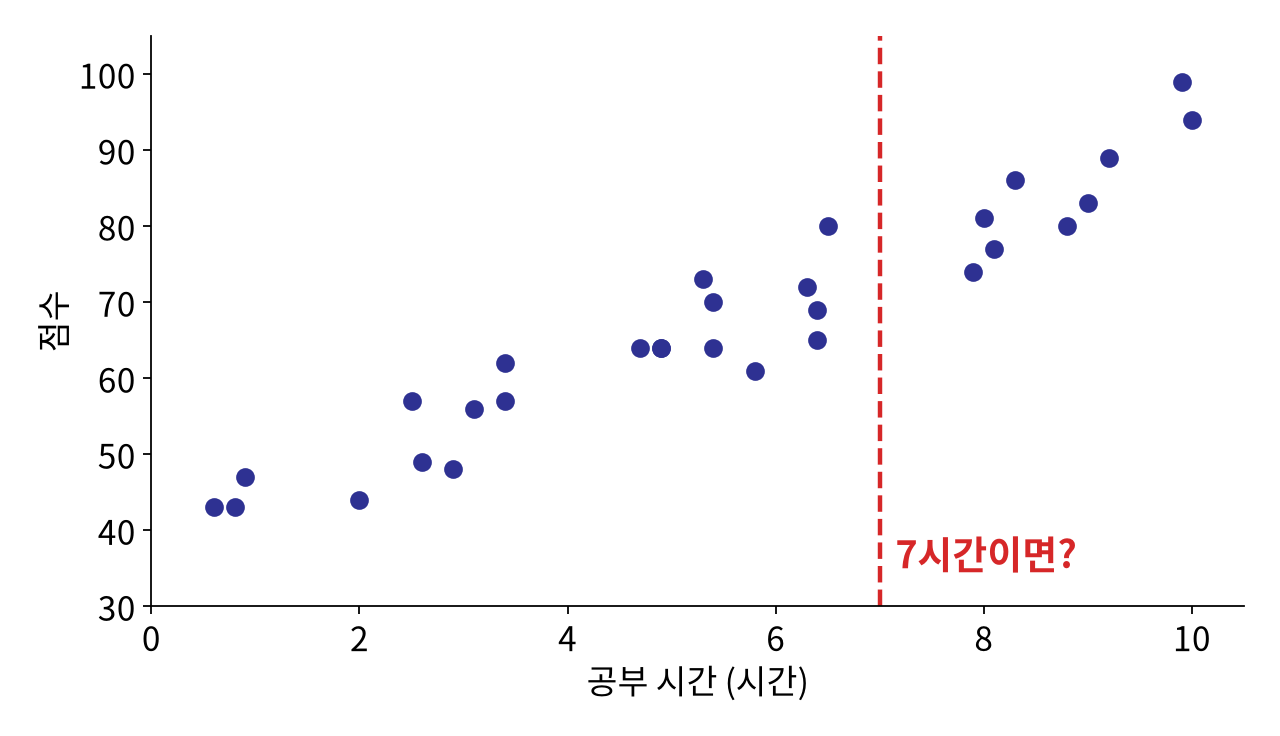
\includegraphics[width=0.62\linewidth]{lr_hook.png}\par\vskip0.3em
{\large 학생 30명의 공부 시간과 점수. \kq{7시간 공부하면 몇 점일까?}}
\vfill
\note{학생 30명의 공부 시간과 시험 점수입니다. 공부를 많이 할수록 점수가 높은 경향이 보입니다. 그러면 7시간 공부한 학생은 몇 점쯤 받을까요? 이렇게 숫자를 예측하는 문제를 회귀라고 하고, 오늘은 가장 기본적인 방법인 선형회귀를 배웁니다.}
\end{frame}

% --- 학습의 정의 (Mitchell)
\begin{frame}{머신러닝이 ``학습한다''는 것은}
\markpage{tpe}
\vfill
\centering
{\Large 작업 \kb{$T$} 에서, 성능 척도 \kb{$P$} 로 쟀을 때,\\[0.3em] 경험 \kb{$E$} 가 쌓일수록 성능이 나아지면\\[0.3em] \kq{``학습한다''}라고 정의한다}\par\vskip1.2em
{\normalsize\color{gray}\itshape ``A computer program is said to learn from experience $E$ with respect to\\ some class of tasks $T$ and performance measure $P$, if its performance\\ at tasks in $T$, as measured by $P$, improves with experience $E$.''}\par\vskip0.8em
{\scriptsize\color{gray} T. Mitchell, \textit{Machine Learning} (1997)}
\vfill
\note{오늘 처음으로 모델을 학습시킵니다. 그 전에 학습이 무엇인지 정의부터 봅시다. 톰 미첼이 1997년 교과서 머신러닝에서 쓴 정의이고, 아래가 영어 원문입니다. 어떤 작업 T에서, 성능 척도 P로 쟀을 때, 경험 E가 쌓일수록 성능이 나아지면 그 프로그램은 학습한다고 정의합니다. 작업, 성능 척도, 경험. 이 세 가지를 정해야 학습을 말할 수 있습니다.}
\end{frame}

% --- T P E 를 오늘 문제에
\begin{frame}{오늘 문제에 대 보면: $T$ · $P$ · $E$}
\vfill
\centering
{\large
\begin{tabular}{rll}
\kb{$T$} & 작업 (task) & 공부 시간으로 시험 점수 맞히기\\[0.6em]
\kb{$P$} & 성능 척도 (performance) & 예측이 평균 몇 점 틀렸나 \quad {\normalsize\color{gray}(에러가 작을수록 좋다)}\\[0.6em]
\kb{$E$} & 경험 (experience) & 학생 30명의 (공부 시간, 점수)
\end{tabular}}\par\vskip1.4em
{\large 데이터를 보고 틀리는 정도를 \kb{줄여 가는 것}이 학습}
\vfill
\note{오늘 문제에 대 보면, 작업 T는 공부 시간으로 시험 점수를 맞히는 것, 성능 척도 P는 예측이 평균 몇 점이나 틀렸는지, 경험 E는 학생 30명의 공부 시간과 점수입니다. 데이터를 보면서 틀리는 정도를 점점 줄여 가는 것, 그게 학습입니다. 그럼 문제를 풀기 전에 무엇을 정해야 하는지 다음 쪽에서 봅니다.}
\end{frame}

% --- 다섯 칸 (옛 01-2 문제 정형화에서 옮김)
\begin{frame}{풀기 전에 정할 것: 다섯 칸}
\markpage{five}
\vfill
\centering
{\large\renewcommand{\arraystretch}{1.25}
\begin{tabular}{rll}
& & \textbf{오늘 문제}\\\hline
\kb{①} & \textbf{한 행}은 무엇? & 학생 한 명 (공부 시간, 점수) \hfill {\normalsize\color{gray}예: (6.4, 65), 이런 행 30개 $= E$}\\
\kb{②} & \textbf{입력} $X$ & 공부 시간 \hfill {\normalsize\color{gray}예측하는 순간 알 수 있는 것만}\\
\kb{③} & \textbf{출력} $y$ & 시험 점수 \hfill {\normalsize\color{gray}숫자면 \kb{회귀}, 범주면 \kb{분류}}\\
\kb{④} & \textbf{평가지표} & 평균 몇 점 틀렸나 \hfill {\normalsize\color{gray}$= P$}\\
\kb{⑤} & \textbf{베이스라인} & 모두에게 평균 점수 67점 $\to$ 평균 \kq{15점} 틀린다
\end{tabular}}\par\vskip1.0em
{\large 모델 점수는 \kb{베이스라인과 비교}해서 읽는다}\\[0.3em]
{\normalsize\color{gray} 프로젝트 1 Abstract (3주차)에 쓸 것이 바로 이 다섯 칸}
\vfill
\note{문제를 풀기 전에 다섯 칸을 채웁니다. 첫째, 한 행, 즉 예시 하나가 무엇인지. 오늘은 학생 한 명의 공부 시간과 점수 한 쌍입니다. 예를 들어 첫 학생은 6.4시간 공부해서 65점을 받았습니다. 표로 놓으면 이게 한 줄이고, 이런 줄이 30개 있습니다. 경험 E는 바로 이 30개 행을 모은 것입니다. 한 행을 학생 한 명으로 할지, 시험 한 번으로 할지에 따라 같은 기록이라도 다른 문제가 됩니다. 둘째, 입력. 예측하는 순간에 실제로 알 수 있는 것만 넣어야 합니다. 시험 전에 공부 시간은 알지만, 시험지를 받고 나서 안 것을 넣으면 답을 미리 보고 맞히는 셈입니다. 셋째, 출력. 점수처럼 숫자를 맞히면 회귀, 합격 불합격처럼 범주 중 하나를 고르면 분류입니다. 넷째, 평가지표. 앞에서 본 성능 척도 P, 평균 몇 점 틀렸나입니다. 다섯째, 베이스라인. 머리를 전혀 안 쓴 답이 몇 점인지입니다. 모든 학생에게 평균 점수 67점이라고 찍으면 평균 15점쯤 틀립니다. 우리 직선이 이것보다 얼마나 나은지가 진짜 성적입니다. 3주차에 내는 프로젝트 1 Abstract에 쓸 것이 바로 이 다섯 칸입니다. 그럼 실제로 무엇을 정하면 학습이 돌아가는지 봅니다.}
\end{frame}

% --- 학습의 뼈대
\begin{frame}{학습의 뼈대: 네 가지만 정하면 된다}
\markpage{recipe}
\vfill
\centering
\recipe{{\small 입력과 정답의 쌍}\\{\small $(x, y)$}}{{\small 예측 함수}\\{\small $h(x)$, 안에 $w$}}{{\small 얼마나 틀렸나}\\{\small 숫자 하나}}{{\small 손실이 줄도록}\\{\small $w$ 를 고친다}}\par\vskip0.6em
{\large 거의 모든 머신러닝 알고리즘은 이 \kb{네 가지의 조합}이다}\\[0.3em]
{\large 오늘 수업이 끝나면 \kb{네 칸을 다 채운다}}\\[0.4em]
{\scriptsize Goodfellow, Bengio \& Courville, \textit{Deep Learning} (2016), \S 5.10, p.~151}
\vfill
\note{지도학습으로 모델을 학습시킬 때 정해야 할 것은 네 가지입니다. 첫째 학습 데이터, 입력과 정답의 쌍입니다. 둘째 예측 모델, 입력을 받아 예측값을 내놓는 함수이고 안에 고칠 수 있는 파라미터 w가 있습니다. 셋째 손실함수, 예측이 정답에서 얼마나 틀렸는지를 숫자 하나로 재는 자입니다. 넷째 최적화 알고리즘, 그 손실이 줄어들도록 w를 고치는 방법입니다. 고치고, 다시 예측하고, 다시 재는 것을 반복합니다. 이건 Goodfellow의 딥러닝 책 5장에서 정리한 틀이고, 거의 모든 알고리즘이 이 네 가지의 조합입니다. 앞으로 배우는 로지스틱회귀, 신경망도 모델과 손실만 바꿔 끼운 것입니다. 오늘 수업에서 이 네 칸을 하나씩 채우고, 끝에서 다시 봅니다.}
\end{frame}


\section{비용}
% --- 모델
\begin{frame}{직선을 긋는다}
\vfill
\centering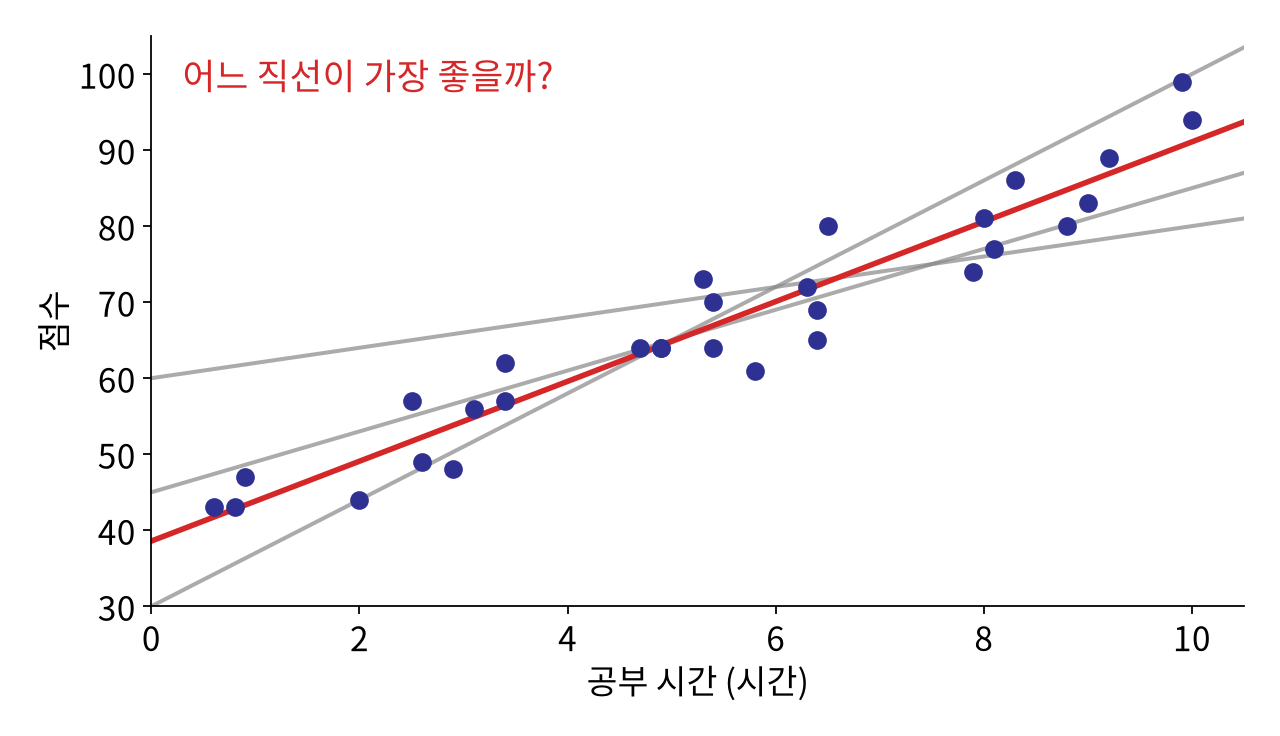
\includegraphics[width=0.47\linewidth]{lr_lines.png}\par\vskip0.3em
{\LARGE\[ h_{\boldsymbol w}(x) = w_0 + w_1 x \]}
{\small $w_0$: 절편 \qquad $w_1$: 기울기 (1시간 더 하면 몇 점 오르나)}
\vfill
\note{점들 사이로 직선을 하나 그어서, 그 직선으로 예측합니다. 직선은 절편 w0와 기울기 w1, 숫자 두 개로 정해집니다. w1은 공부를 1시간 더 하면 점수가 몇 점 오르는지를 뜻합니다. 그런데 그을 수 있는 직선은 무수히 많습니다. 어느 직선이 가장 좋은지 기준이 필요합니다.}
\end{frame}

% --- 비용
\begin{frame}{오차를 제곱해서 평균: 비용 $J$}
\markpage{cost}
\vfill
\begin{columns}[c]
\begin{column}{0.52\textwidth}\centering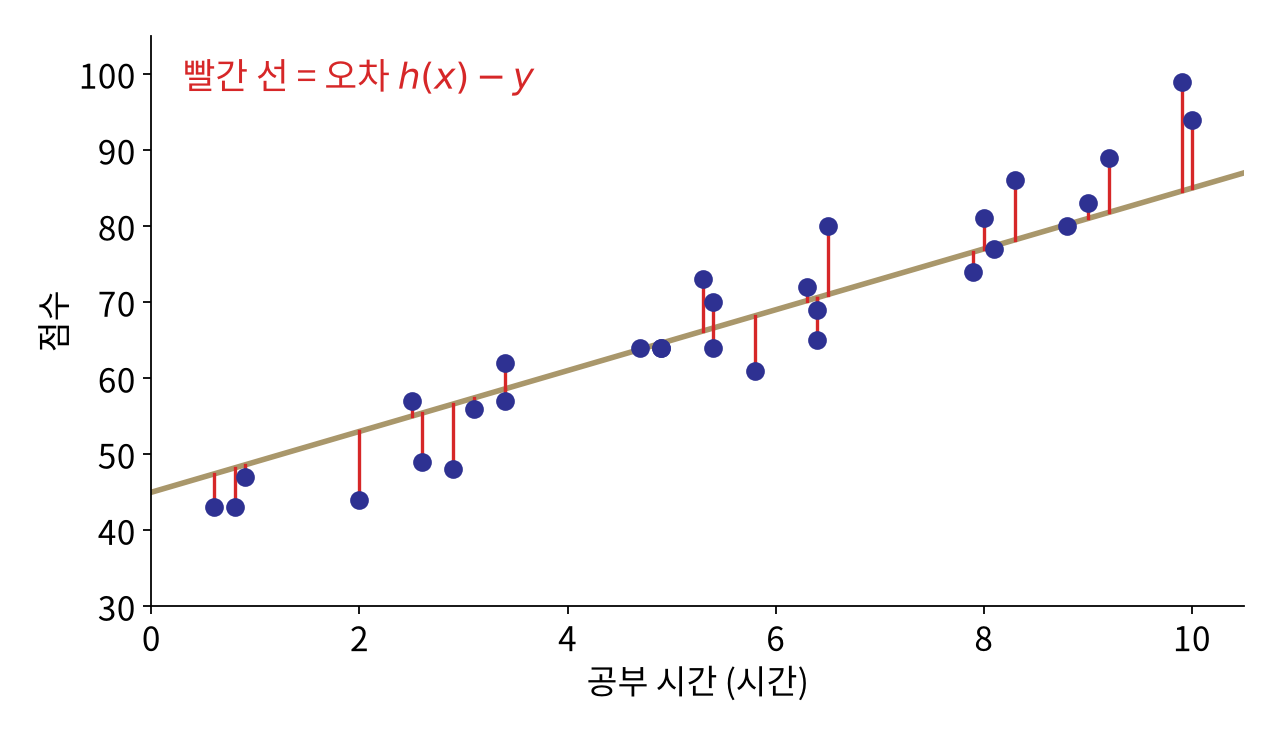
\includegraphics[width=\linewidth]{lr_residuals.png}\end{column}
\begin{column}{0.44\textwidth}
{\large\[ J(\boldsymbol w) = \frac{1}{2m}\sum_{i=1}^{m}\big(h_{\boldsymbol w}(x^{(i)}) - y^{(i)}\big)^2 \]}\vskip0.4em
{\small $m$: 데이터 수 (30명) \quad 빨간 선: 오차}\\[0.5em]
{\small 제곱: 음수 오차와 양수 오차가 상쇄되지 않게}\\[0.2em]
{\small $\frac12$: 미분할 때 2와 약분되라고 붙인 것}
\end{column}
\end{columns}
\vfill
\note{기준은 오차입니다. 각 학생마다 직선이 예측한 점수와 실제 점수의 차이, 빨간 선이 오차입니다. 오차를 그냥 더하면 위아래가 상쇄되니까 제곱해서 더하고, 데이터 수로 나눠 평균을 냅니다. 앞의 2분의 1은 미분할 때 지수 2와 약분되라고 붙인 것입니다. 이 값을 비용 J라고 부르고, J가 가장 작은 직선이 가장 좋은 직선입니다.}
\end{frame}

% --- 그릇
\begin{frame}{$J$ 는 그릇 모양}
\vfill
\centering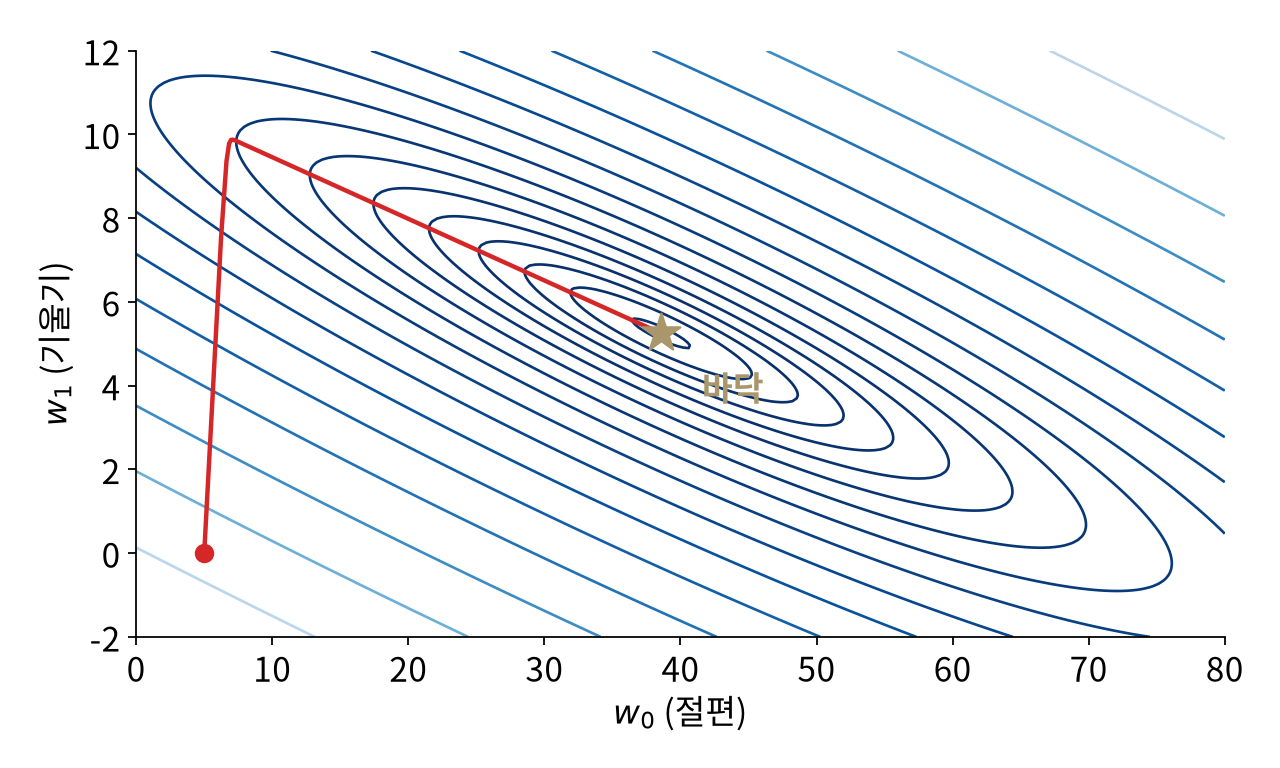
\includegraphics[width=0.8\linewidth]{lr_bowl.png}\par\vskip0.1em
{\small\renewcommand{\arraystretch}{1.1}\setlength{\tabcolsep}{7pt}
\begin{tabular}{l|rrrr|rrr}
걸음 & 0 & 1 & 2 & 3 & 100 & 1000 & 4000\\\hline
$(w_0,\ w_1)$ & (5, 0) & (6.2, 7.6) & (6.6, 9.4) & (6.8, 9.8) & (17.0, 8.4) & (38.0, 5.3) & \kb{(38.6, 5.3)}\\
$J$ & 2046 & 224 & 119 & 112 & 56.7 & 9.56 & \kb{9.52}
\end{tabular}}\par\vskip0.3em
{\small 걸음마다 그 자리에서 \kq{가장 가파른 내리막} (등고선에 수직), 골짜기에 들어서면 아주 조금씩 ($\eta = 0.02$)}
\vfill
\note{w0와 w1을 바꿔 가며 J를 계산하면 이렇게 그릇 모양이 됩니다. 등고선 지도로 그렸는데, 가운데 별이 바닥, 즉 J가 가장 작은 곳입니다. 그릇의 바닥은 하나뿐이라서, 어디서 출발하든 내리막을 따라가면 같은 바닥에 도착합니다. 빨간 선이 경사하강법이 실제로 걸어간 길입니다. 가로와 세로 눈금을 같게 그렸습니다. 그래야 걸음 방향이 등고선에 수직으로 보입니다. 경사하강법은 매 걸음 그 자리에서 가장 가파른 내리막, 즉 등고선에 수직인 방향으로 갑니다. 첫 걸음에 J가 2046에서 224로 크게 줄고, w1이 0에서 7.6으로 크게 움직입니다. 공부 시간 x가 곱해지는 w1 쪽이 훨씬 가파르기 때문입니다. 세 걸음 만에 길쭉한 골짜기 바닥에 들어서면, 그 다음부터는 골짜기를 따라 아주 조금씩 갑니다. 100걸음에 J가 56.7, 1000걸음에 9.56, 4000걸음에 9.52로 바닥에 닿습니다. 골짜기가 좁고 길수록 경사하강법이 느려지는 이유입니다.}
\end{frame}

\section{경사하강법}
% --- 경사하강법
% --- 미분 준비: 연쇄 법칙
\begin{frame}{미분 준비: 연쇄 법칙 (chain rule)}
\markpage{chain}
\vfill
\centering
{\LARGE\[ \frac{d}{dw}\Big[\textcolor{ksared}{\big(}\textcolor{ksablue}{g(w)}\textcolor{ksared}{\big)^{n}}\Big] = \textcolor{ksared}{n\big(}\textcolor{ksablue}{g(w)}\textcolor{ksared}{\big)^{n-1}}\cdot \textcolor{ksablue}{g'(w)} \]}\vskip0.4em
{\LARGE\[ \frac{d}{dw}\Big[\textcolor{ksared}{f\big(}\textcolor{ksablue}{g(w)}\textcolor{ksared}{\big)}\Big] = \textcolor{ksared}{f'\big(}\textcolor{ksablue}{g(w)}\textcolor{ksared}{\big)}\;\textcolor{ksablue}{g'(w)} \]}\vskip0.4em
{\normalsize \textcolor{ksared}{\textbf{빨강}}: 바깥을 미분 (제곱이면 \textbf{지수 2 가 앞으로 내려온다}) \qquad \textcolor{ksablue}{\textbf{파랑}}: 안쪽 $g$ 와 안쪽을 미분한 값}\vskip0.8em
{\large 예: \; $\dfrac{d}{dw}(3w+1)^{\textcolor{ksared}{2}} = \textcolor{ksared}{2}(3w+1)\cdot \textcolor{ksablue}{3}$ \quad {\normalsize\color{gray}(펼쳐서 $9w^2+6w+1$ 을 미분한 $18w+6$ 과 같다)}}
\vfill
\note{기울기를 구하기 전에 미분 규칙 하나만 준비합니다. 연쇄 법칙입니다. 함수 안에 또 함수가 들어 있으면, 바깥을 미분하고 안쪽을 미분한 값을 곱합니다. 위 식은 n제곱일 때, 아래 식은 일반적인 경우입니다. 빨간색이 바깥, 파란색이 안쪽입니다. 우리가 쓸 건 제곱입니다. 제곱을 미분하면 빨간 지수 2가 앞으로 내려오고, 여기에 안쪽 g를 w로 미분한 값을 파란색으로 곱합니다. 예를 들어 3w 더하기 1의 제곱을 미분하면 2 곱하기 3w 더하기 1, 곱하기 안쪽의 미분 3입니다. 펼쳐서 9w 제곱 더하기 6w 더하기 1을 미분해도 18w 더하기 6으로 같습니다. 다음 쪽에서 이 규칙을 그대로 J에 씁니다.}
\end{frame}

\begin{frame}{경사하강법: 기울기 반대로 한 걸음}
\markpage{gd}
\centering
{\Large\[ w_j \;\leftarrow\; w_j - \eta\,\frac{\partial J}{\partial w_j} \]}\vskip-0.6em
{\small $\eta$: 학습률 (한 걸음의 크기), 예: $\eta = 0.1$ \qquad 기울기 $\partial J/\partial w_j$ 는 연쇄 법칙 \pref{chain} 으로}\vskip0.3em
\begin{columns}[T]
\begin{column}{0.49\textwidth}
\begin{align*}
\frac{\partial J}{\partial w_0}
&= \frac{1}{2m}\sum\nolimits_{i=1}^{m}\frac{\partial}{\partial w_0}\big(w_0 + w_1 x^{(i)} - y^{(i)}\big)^{\textcolor{ksared}{2}}\\
&= \frac{1}{\textcolor{ksared}{2}m}\sum\nolimits_{i=1}^{m}\textcolor{ksared}{2}\big(w_0 + w_1 x^{(i)} - y^{(i)}\big)\cdot\textcolor{ksablue}{1}\\
&= \frac{1}{m}\sum\nolimits_{i=1}^{m}\big(h(x^{(i)}) - y^{(i)}\big)
\end{align*}
\end{column}
\begin{column}{0.49\textwidth}
\begin{align*}
\frac{\partial J}{\partial w_1}
&= \frac{1}{2m}\sum\nolimits_{i=1}^{m}\frac{\partial}{\partial w_1}\big(w_0 + w_1 x^{(i)} - y^{(i)}\big)^{\textcolor{ksared}{2}}\\
&= \frac{1}{\textcolor{ksared}{2}m}\sum\nolimits_{i=1}^{m}\textcolor{ksared}{2}\big(w_0 + w_1 x^{(i)} - y^{(i)}\big)\cdot\textcolor{ksablue}{x^{(i)}}\\
&= \frac{1}{m}\sum\nolimits_{i=1}^{m}\big(h(x^{(i)}) - y^{(i)}\big)\,\textcolor{ksablue}{x^{(i)}}
\end{align*}
\end{column}
\end{columns}\vskip0.2em
{\small \textcolor{ksared}{\textbf{빨강}}: 지수 2 가 앞으로 내려와 $\frac12$ 과 약분 \pref{cost} \qquad
\textcolor{ksablue}{\textbf{파랑}}: 괄호 안을 미분한 값 ($w_0$ 로는 $1$, $w_1$ 로는 $x^{(i)}$)}
\note{바닥을 찾는 방법이 경사하강법입니다. 지금 위치에서 J가 늘어나는 방향, 즉 기울기를 구해서 그 반대로 학습률 에타만큼 걷습니다. 기울기를 직접 구해 봅시다. 왼쪽이 w0, 오른쪽이 w1입니다. 둘 다 같은 순서입니다. 제곱을 미분하면 빨간 지수 2가 앞으로 내려옵니다. 이 2가 J 앞에 붙여 둔 2분의 1과 약분됩니다. 2분의 1을 붙인 이유가 이것입니다. 그리고 괄호 안을 미분한 값을 곱합니다. 파란색입니다. 괄호 안을 w0로 미분하면 1, w1로 미분하면 x입니다. 그래서 w0 쪽 기울기는 오차의 평균, w1 쪽은 오차 곱하기 입력의 평균이 됩니다. 예측이 크게 틀린 학생일수록, 그리고 공부 시간이 긴 학생일수록 w1을 크게 고칩니다. 실습에서 이 두 줄을 직접 구현합니다.}
\end{frame}

% --- 학습률
\begin{frame}{학습률은 적당히}
\vfill
\centering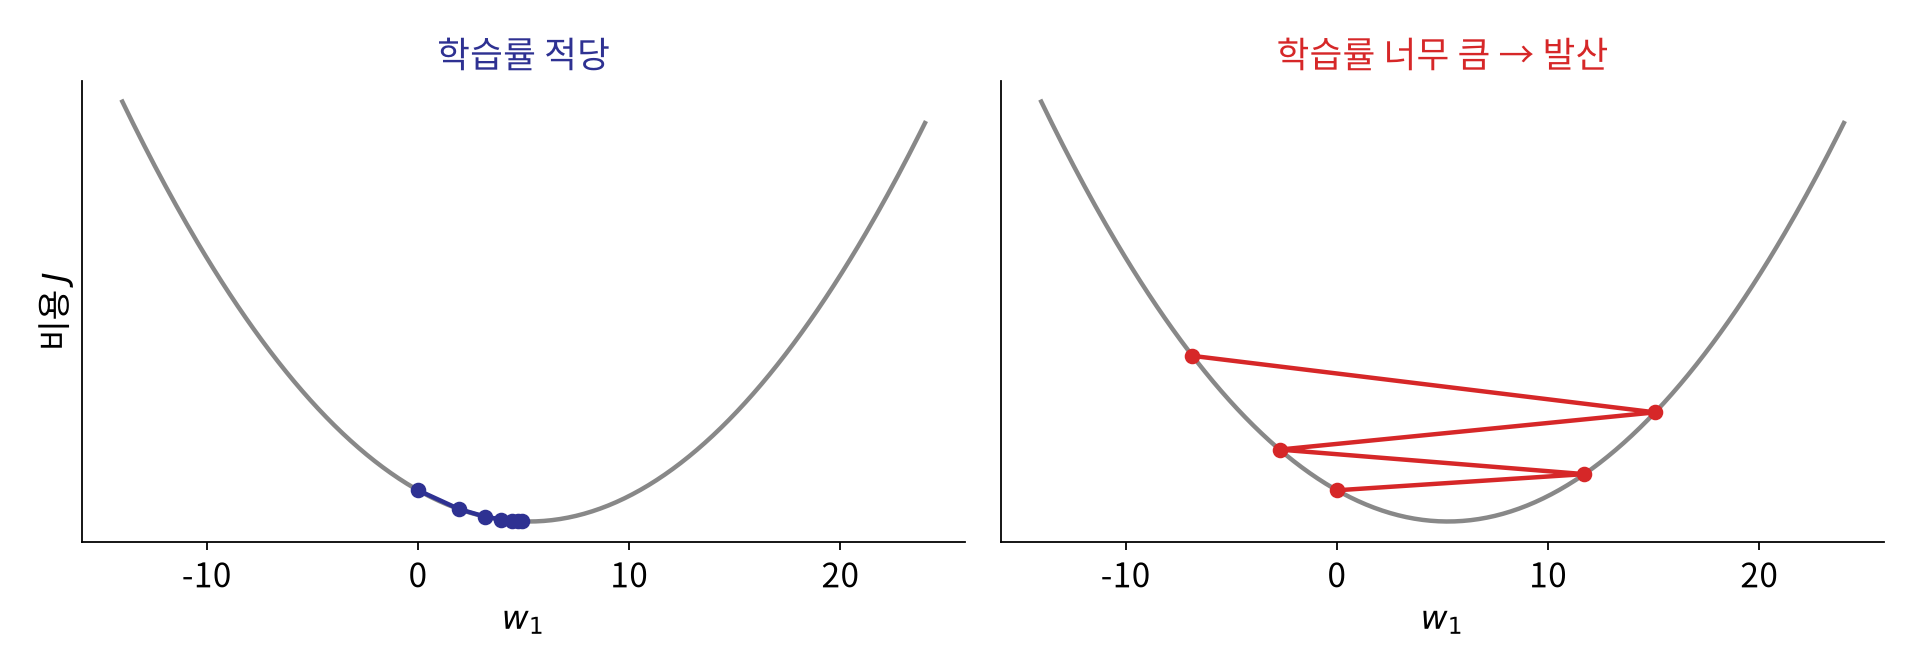
\includegraphics[width=0.86\linewidth]{lr_alpha.png}\par\vskip0.3em
{\large 너무 작으면 느리고, \kq{너무 크면 바닥을 건너뛰며 튕겨 나간다}}
\vfill
\note{학습률이 적당하면 왼쪽처럼 바닥으로 차근차근 내려갑니다. 그런데 너무 크면 오른쪽처럼 바닥을 건너뛰어 반대편으로 가고, 매번 더 높은 곳에 떨어지면서 튕겨 나갑니다. 이걸 발산이라고 합니다. 너무 작으면 바닥까지 한참 걸리고요. 그래서 학습률은 적당히 골라야 합니다.}
\end{frame}

% --- 같은 그릇, 학습률 네 가지
\begin{frame}{같은 그릇, 학습률 네 가지}
\vfill
\centering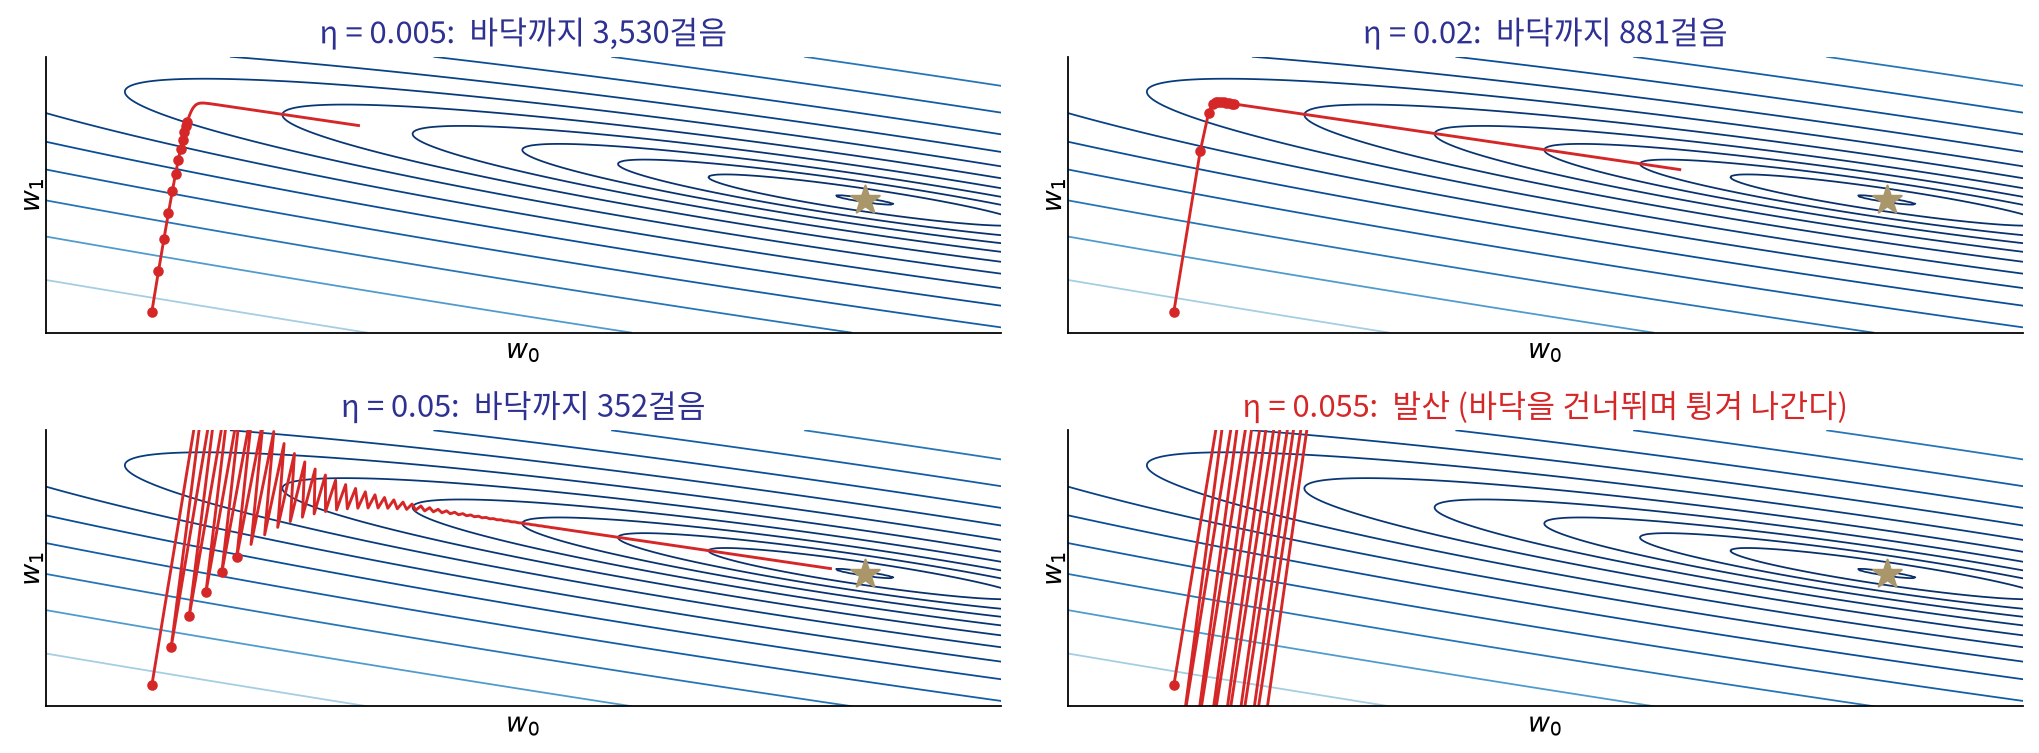
\includegraphics[width=0.94\linewidth]{lr_rates.png}\par\vskip0.3em
{\small 같은 출발점 $(5, 0)$, 빨간 선 = 처음 300걸음 (점 = 처음 12걸음). 걸음 수 = $J$ 가 바닥값의 1\% 안에 들 때까지}\\[0.3em]
{\large 이 데이터는 $\eta$ 를 \kq{0.053 넘게 키울 수 없다}: 가파른 $w_1$ 쪽에서 튕겨 나간다}
\vfill
\note{같은 그릇, 같은 출발점에서 학습률만 바꿔 봤습니다. 빨간 선은 처음 300걸음입니다. 0.005면 300걸음이 지나도 아직 골짜기 입구이고, 바닥까지 3천5백 걸음이 넘게 걸립니다. 0.02면 880걸음쯤입니다. 0.05로 키우면 처음에 가파른 w1 방향으로 위아래 지그재그를 하다가 골짜기에 들어서고, 350걸음이면 바닥입니다. 그런데 0.055로 조금만 더 키우면 지그재그가 점점 커지면서 튕겨 나갑니다. 발산입니다. 이 데이터에서는 학습률을 0.053보다 키울 수 없습니다. 가파른 w1 방향이 한계를 정하고, 완만한 골짜기 방향은 그 작은 학습률로 천천히 갈 수밖에 없습니다. 그래서 학습률만으로는 빨라지는 데 한계가 있습니다. 그릇 자체를 동그랗게 만드는 방법을 다음 쪽에서 봅니다.}
\end{frame}

% --- 왜 w1 쪽만 가파른가
\begin{frame}{왜 $w_1$ 쪽만 가파를까: $w_0$ 에는 1, $w_1$ 에는 $x$ 가 곱해진다}
\vfill
\centering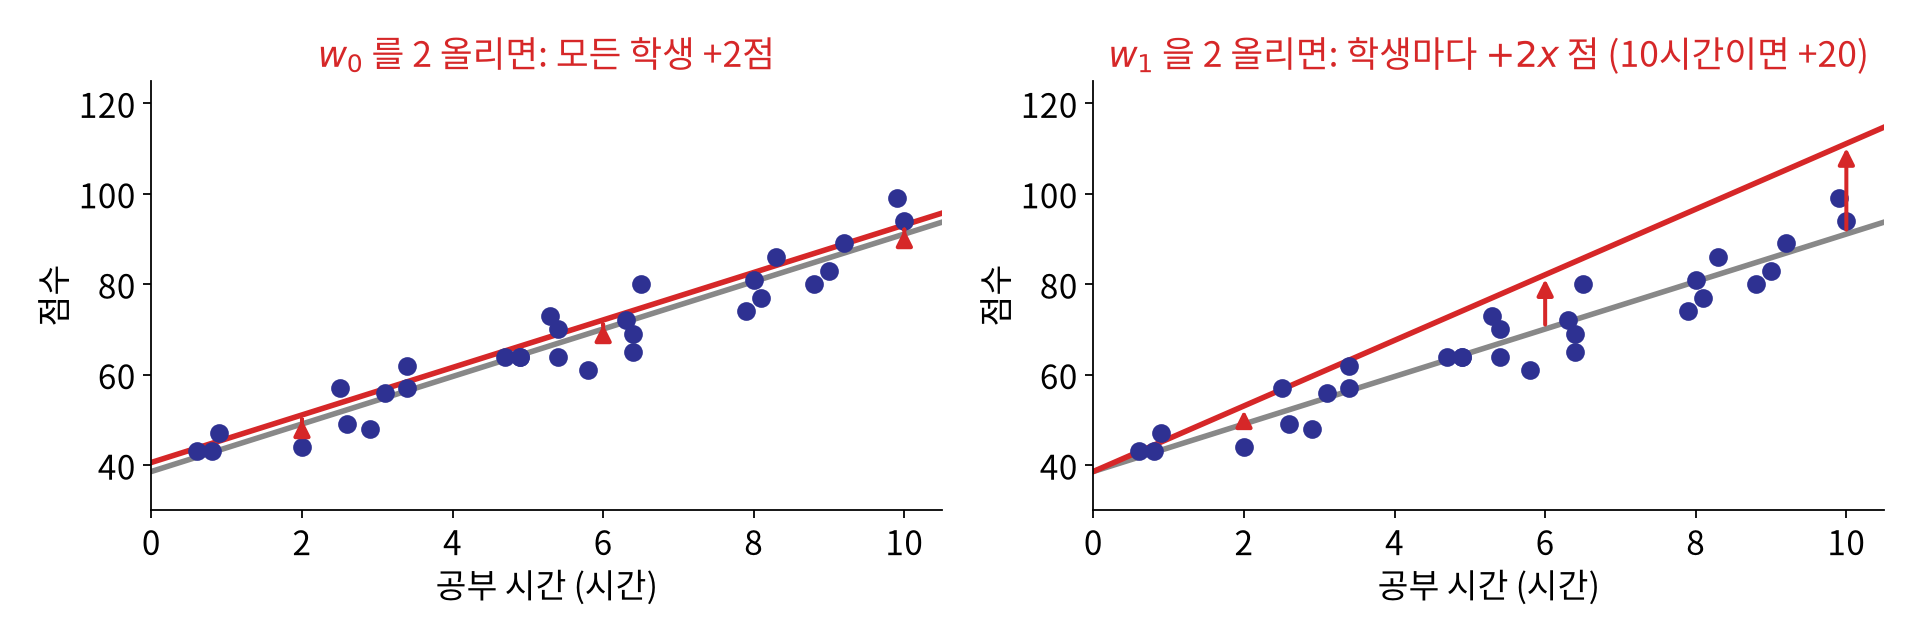
\includegraphics[width=0.74\linewidth]{lr_nudge.png}\par\vskip0.1em
{\large $h = w_0 \cdot \textcolor{ksablue}{1} + w_1 \cdot \textcolor{ksared}{x}$}\\[0.3em]
{\normalsize 출발점 $(5, 0)$ 의 기울기: \; $\partial J/\partial w_0 = -62$ (오차 $\times \textcolor{ksablue}{1}$) \quad vs \quad $\partial J/\partial w_1 = \kq{-378}$ (오차 $\times \textcolor{ksared}{x}$), 6배}\\[0.3em]
{\normalsize 같은 $\eta$ 로 걸으면 $w_1$ 은 \kq{크게 튀고} ($\eta$ 를 못 키움), $w_0$ 는 \kb{거의 안 움직인다} (느림)}
\vfill
\note{왜 w1 쪽만 이렇게 가파를까요? 직선 식을 다시 보면 w0에는 1이 곱해지고, w1에는 공부 시간 x가 곱해집니다. 왼쪽 그림처럼 w0를 2 올리면 모든 학생의 예측이 똑같이 2점 오릅니다. 오른쪽처럼 w1을 2 올리면 학생마다 2 곱하기 x점이 오릅니다. 2시간 공부한 학생은 4점, 10시간 공부한 학생은 20점입니다. 같은 만큼 바꿔도 w1 쪽이 J를 훨씬 크게 흔듭니다. 실제로 출발점에서 기울기를 재 보면 w0 쪽은 마이너스 62, w1 쪽은 마이너스 378로 6배 차이가 납니다. 기울기 식에서 w1 쪽에만 x가 곱해지기 때문입니다. 그래서 같은 학습률로 걸으면 w1은 크게 튀고, 튀지 않게 학습률을 줄이면 이번에는 w0가 거의 움직이지 않습니다. 이게 경사하강법이 느린 이유입니다. 해결책은 x의 크기를 1과 비슷하게 맞추는 것, 다음 쪽의 표준화입니다.}
\end{frame}

% --- 입력 표준화
\begin{frame}{그릇을 동그랗게: 입력 표준화 (z-score normalization)}
\markpage{scaling}
\vfill
\centering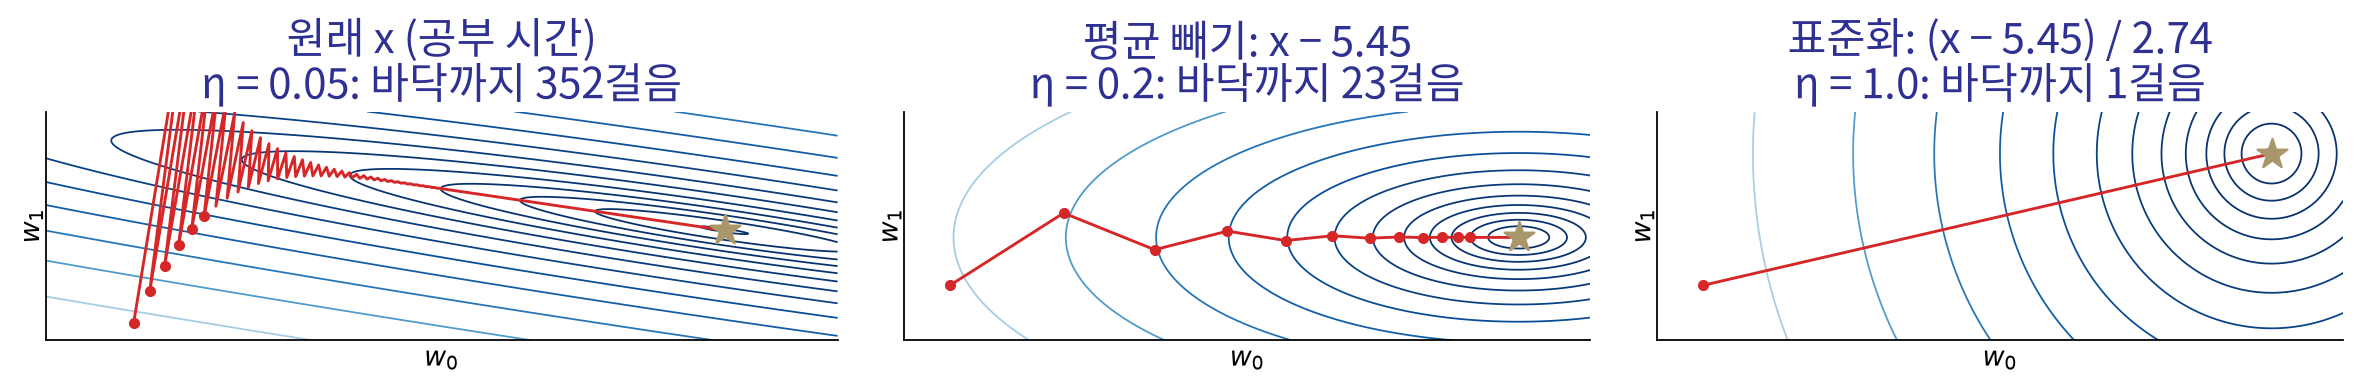
\includegraphics[width=\linewidth]{lr_scaling.png}\par\vskip0.4em
{\large $x' = \dfrac{x - \mu}{\sigma} = \dfrac{x - 5.45}{2.74}$ \qquad {\normalsize $\mu$: 평균, $\sigma$: 표준편차 $\to$ $x'$ 는 $\mu = 0$, $\sigma = 1$}}\\[0.5em]
{\normalsize 예측할 때도 같은 변환: 7시간 $\to 0.57 \to 67.17 + 14.41 \times 0.57 = \kb{75.3점}$ (같은 답)}\\[0.3em]
{\small\color{gray} $\mu$ 빼기: $w_0$, $w_1$ 이 따로 논다 \quad $\sigma$ 로 나누기: 두 방향의 가파르기가 같아진다 \quad 실습은 01-3}
\vfill
\note{학습률을 아무리 골라도 352걸음이 한계였습니다. 그릇이 비스듬하고 길쭉하기 때문입니다. 원인은 입력 x에 있습니다. 앞에서 본 것처럼 x가 1보다 훨씬 커서 w1 쪽만 가파르고, 또 공부 시간의 평균이 5.45시간이라 0에서 멀리 떨어져 있어서, w0를 조금 바꾸면 w1의 가장 좋은 값도 같이 바뀝니다. 두 축이 얽혀서 그릇이 비스듬해집니다. 가운데 그림처럼 x에서 평균을 빼면 그릇이 똑바로 서고, 학습률을 0.2까지 올릴 수 있어서 23걸음이면 바닥입니다. 오른쪽처럼 평균을 빼고 표준편차 2.74로 나누면 두 방향의 가파르기가 같아져서 그릇이 동그래지고, 학습률 1로 한 걸음 만에 바닥에 닿습니다. 이걸 표준화라고 합니다. 주의할 점이 하나 있습니다. 표준화한 x로 학습했으면 예측할 때도 같은 평균과 표준편차로 바꿔서 넣어야 합니다. 7시간이면 7 빼기 5.45를 2.74로 나눈 0.57을 넣고, 67.17 더하기 14.41 곱하기 0.57, 75.3점으로 원래 직선과 같은 답이 나옵니다. 모델이 바뀐 게 아니라 눈금만 바꾼 것이니까요. 다음 시간 데이터 다루기에서 직접 해 봅니다.}
\end{frame}

% --- 결과
\begin{frame}{바닥에 도착하면}
\vfill
\centering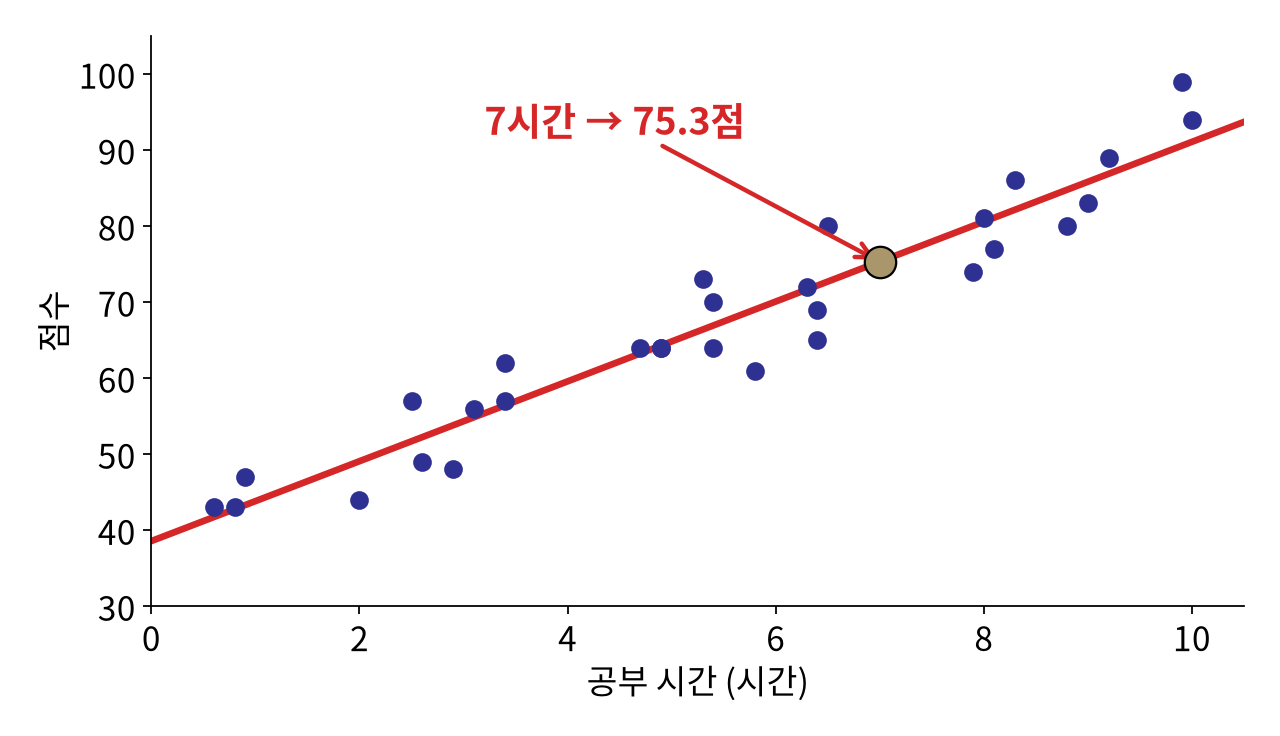
\includegraphics[width=0.6\linewidth]{lr_fit.png}\par\vskip0.3em
{\large $h(x) = 38.6 + 5.25\,x$ \qquad \kq{7시간 $\to$ 75.3점}}
\vfill
\note{바닥에 도착하면 절편 38.6, 기울기 5.25인 직선이 나옵니다. 공부를 1시간 더 할 때마다 약 5점씩 오른다는 뜻입니다. 7을 넣으면 75.3점. 처음 질문의 답입니다.}
\end{frame}

% --- 손으로 풀기: 문제
\begin{frame}{한 문제, 두 가지 풀이}
\vfill
\centering
{\large 점 $(1,2),\ (2,4),\ (3,5)$ 에 직선 $h(x) = w_0 + w_1 x$ 를 맞춘다}\vskip0.8em
\begin{tabular}{c|ccc}
$x$ & 1 & 2 & 3 \\ \hline
$y$ & 2 & 4 & 5
\end{tabular}\vskip0.8em
{\large \kq{$J$ 가 가장 작은 $w_0,\ w_1$ 은?}}\vskip0.6em
{\small 풀이 A: 경사하강법으로 걸어서 \qquad 풀이 B: 식을 풀어서 바로}
\vfill
\note{작은 문제 하나를 두 가지 방법으로 풉니다. 점은 세 개, 1에 2, 2에 4, 3에 5입니다. 직선 h는 w0 더하기 w1 곱하기 x이고, 비용 J가 가장 작은 w0와 w1을 찾습니다. 하나는 방금 배운 경사하강법으로 한 걸음씩 걸어서, 다른 하나는 식을 세워서 바로 풉니다. 같은 답이 나오는지 보세요.}
\end{frame}

% --- 풀이 A ①
\begin{frame}{풀이 A ① 첫 걸음: 오차와 기울기 계산 ($\eta = 0.1$, $w_0 = w_1 = 0$ 에서 출발)}
\markpage{solA}
\vfill
\centering
{\large\renewcommand{\arraystretch}{1.2}
\begin{tabular}{c|cc|c|c|c}
$i$ & $x$ & $y$ & 예측 $h = 0 + 0 \cdot x$ & 오차 $e = h - y$ & $e \cdot x$\\\hline
1 & 1 & 2 & 0 & $-2$ & $-2$\\
2 & 2 & 4 & 0 & $-4$ & $-8$\\
3 & 3 & 5 & 0 & $-5$ & $-15$\\\hline
\multicolumn{4}{r|}{합} & $-11$ & $-25$
\end{tabular}}\vskip0.8em
{\large
$\dfrac{\partial J}{\partial w_0} = \dfrac{1}{m}\sum e = \dfrac{-11}{3} = \kb{-3.67}$ \qquad
$\dfrac{\partial J}{\partial w_1} = \dfrac{1}{m}\sum e\,x = \dfrac{-25}{3} = \kb{-8.33}$}\\[0.4em]
{\small\color{gray} 기울기 식은 \pref{gd}, $m = 3$ (점 3개)}
\vfill
\note{경사하강법으로 풉니다. 학습률은 0.1, 출발점은 w0도 w1도 0입니다. 표를 만들어 한 줄씩 채우면 실수가 없습니다. 지금 직선은 0 더하기 0 곱하기 x라서 예측은 모두 0입니다. 오차는 예측 빼기 정답이니 마이너스 2, 마이너스 4, 마이너스 5입니다. 오차 곱하기 x는 마이너스 2, 마이너스 8, 마이너스 15입니다. 이제 앞에서 구한 기울기 식에 넣습니다. w0 기울기는 오차의 평균, 합 마이너스 11을 3으로 나눈 마이너스 3.67. w1 기울기는 오차 곱하기 x의 평균, 마이너스 25를 3으로 나눈 마이너스 8.33입니다.}
\end{frame}

% --- 풀이 A ②
\begin{frame}{풀이 A ② 한 걸음 가고, 같은 계산을 반복}
\vfill
\begin{columns}[c]
\begin{column}{0.56\textwidth}
{\small
\begin{align*}
w_0 &\leftarrow w_0 - \eta\,\tfrac{\partial J}{\partial w_0} = 0 - 0.1 \times (-3.67) = \textcolor{ksablue}{0.37}\\
w_1 &\leftarrow w_1 - \eta\,\tfrac{\partial J}{\partial w_1} = 0 - 0.1 \times (-8.33) = \textcolor{ksablue}{0.83}\\[0.5em]
\text{확인:}\ h &= 0.37 + 0.83\,x = 1.20,\ 2.03,\ 2.87\\
e &= h - y = -0.80,\ -1.97,\ -2.13\\
J &= \tfrac{1}{2 \cdot 3}\big(0.80^2 + 1.97^2 + 2.13^2\big) = \textcolor{ksablue}{1.51}
\end{align*}}
{\small $J$: 7.50 $\to$ 1.51. \; 둘째 걸음: 새 $w$ 로 \pref{solA} 의 표를 다시}
\end{column}
\begin{column}{0.44\textwidth}
\centering
{\normalsize\renewcommand{\arraystretch}{1.15}
\begin{tabular}{r|rrr}
걸음 & $w_0$ & $w_1$ & $J$ \\ \hline
0 & 0 & 0 & 7.50 \\
1 & 0.37 & 0.83 & 1.51 \\
2 & 0.53 & 1.20 & 0.32 \\
3 & 0.60 & 1.37 & 0.09 \\
10 & 0.66 & 1.50 & 0.028 \\
400 & 0.667 & 1.500 & 0.0278
\end{tabular}}\par\vskip0.5em
{\large \kq{수백 걸음 뒤}\\ $w_0 \approx 0.667,\ w_1 \approx 1.5$}
\end{column}
\end{columns}
\vfill
\note{기울기의 반대 방향으로 학습률만큼 갑니다. w0는 0 빼기 0.1 곱하기 마이너스 3.67, 0.37입니다. 마이너스에 마이너스라 더해집니다. w1은 0 빼기 0.1 곱하기 마이너스 8.33, 0.83입니다. 잘 갔는지 확인해 봅시다. 새 직선으로 예측하면 1.20, 2.03, 2.87이고 오차는 마이너스 0.80, 마이너스 1.97, 마이너스 2.13입니다. 제곱해서 더하고 6으로 나누면 J는 1.51, 7.50에서 줄었습니다. 둘째 걸음은 새 w로 앞 쪽의 표를 다시 채우면 됩니다. 이렇게 반복하면 오른쪽 표처럼 J가 줄고, 10걸음에서 거의 다 왔고, 400걸음 뒤에는 w0 0.667, w1 1.5에 도착합니다.}
\end{frame}

% --- 풀이 B ①
\begin{frame}{풀이 B ① 바닥에서는 기울기가 0: 식 두 개 세우기}
\markpage{solB}
\vfill
\begin{columns}[c]
\begin{column}{0.66\textwidth}
{\normalsize
\begin{align*}
\frac{\partial J}{\partial w_0} = \frac{1}{m}\sum (w_0 + w_1 x - y) &= 0 && \text{기울기 \pref{gd}}\\
\sum w_0 + w_1 \sum x - \sum y &= 0 && \times m\text{, 합을 나눔}\\
\textcolor{ksablue}{3\,w_0 + 6\,w_1} &\textcolor{ksablue}{= 11} && \textstyle\sum w_0 = m w_0 = 3 w_0\\[0.6em]
\frac{\partial J}{\partial w_1} = \frac{1}{m}\sum (w_0 + w_1 x - y)\,x &= 0\\
w_0 \sum x + w_1 \sum x^2 - \sum xy &= 0 && \times m\text{, } x \text{ 를 곱해 펼침}\\
\textcolor{ksablue}{6\,w_0 + 14\,w_1} &\textcolor{ksablue}{= 25}
\end{align*}}
\end{column}
\begin{column}{0.3\textwidth}
\centering
{\normalsize\renewcommand{\arraystretch}{1.2}
\begin{tabular}{cc|cc}
$x$ & $y$ & $x^2$ & $xy$\\\hline
1 & 2 & 1 & 2\\
2 & 4 & 4 & 8\\
3 & 5 & 9 & 15\\\hline
\kb{6} & \kb{11} & \kb{14} & \kb{25}
\end{tabular}}\par\vskip0.3em
{\small 마지막 줄 = 합 $\sum$}
\end{column}
\end{columns}
\vfill
\note{이번에는 걷지 않고 바닥의 조건을 바로 씁니다. 바닥에서는 두 기울기가 모두 0입니다. 첫 식, w0 기울기를 0으로 놓습니다. 양변에 m을 곱하고, 합을 항마다 나눠 쓰면 w0의 합 더하기 w1 곱하기 x의 합 빼기 y의 합이 0입니다. w0는 점마다 같으니 w0를 세 번 더한 3 w0입니다. 오른쪽 표에서 x의 합 6, y의 합 11을 넣으면 3 w0 더하기 6 w1은 11. 둘째 식, w1 기울기도 0으로 놓고 괄호에 x를 곱해 펼치면 w0 곱하기 x의 합, w1 곱하기 x 제곱의 합, xy의 합이 나옵니다. 표에서 6, 14, 25를 넣으면 6 w0 더하기 14 w1은 25입니다. 미지수 두 개, 식 두 개입니다.}
\end{frame}

% --- 풀이 B ②
\begin{frame}{풀이 B ② 연립방정식 풀기}
\vfill
{\large
\begin{align*}
3\,w_0 + 6\,w_1 &= 11 && \cdots (1)\\
6\,w_0 + 14\,w_1 &= 25 && \cdots (2)\\[0.4em]
(6 w_0 + 14 w_1) - (6 w_0 + 12 w_1) &= 25 - 22 && (2) - 2 \times (1)\\
2\,w_1 &= 3 \;\Rightarrow\; \textcolor{ksablue}{w_1 = 1.5}\\[0.4em]
3\,w_0 + 6 \times 1.5 &= 11 && (1) \text{ 에 대입}\\
3\,w_0 &= 2 \;\Rightarrow\; \textcolor{ksablue}{w_0 = 2/3 \approx 0.667}
\end{align*}}
\centering{\normalsize 확인: $h = 2.17,\ 3.67,\ 5.17$, \quad $J = 0.0278$ (풀이 A 400걸음과 같다)}\\[0.3em]{\small\color{gray} 같은 두 식을 행렬로 쓰면 정규방정식 $\mathbf{w} = (X^\top X)^{-1} X^\top \mathbf{y}$, 유도는 다음 쪽}

\vfill
\note{식 두 개를 풉니다. 1번 식에 2를 곱하면 6 w0 더하기 12 w1은 22입니다. 2번 식에서 이걸 빼면 w0가 지워지고 2 w1은 3, w1은 1.5입니다. 이 값을 1번 식에 넣으면 3 w0 더하기 9가 11, 3 w0는 2, w0는 3분의 2, 약 0.667입니다. 확인해 보면 예측은 2.17, 3.67, 5.17이고 J는 0.0278, 풀이 A가 400걸음 걸어서 도착한 값과 같습니다. 같은 두 식을 행렬로 쓰면 정규방정식이 됩니다. 다음 쪽에서 유도합니다.}
\end{frame}

% --- 정규방정식 유도
\begin{frame}{정규방정식은 어디서 오나: 풀이 B 를 행렬로}
\markpage{normal}
\vfill
\begin{columns}[c]
\begin{column}{0.64\textwidth}
{\normalsize
\begin{align*}
X\mathbf{w} &= \begin{pmatrix} w_0 + w_1 \cdot 1\\ w_0 + w_1 \cdot 2\\ w_0 + w_1 \cdot 3\end{pmatrix} && \text{예측 세 개}\\
\mathbf{e} &= X\mathbf{w} - \mathbf{y} && \text{오차}\\
\begin{pmatrix} \partial J/\partial w_0\\ \partial J/\partial w_1\end{pmatrix}
&= \frac{1}{m}\begin{pmatrix} \sum e \cdot \textcolor{ksablue}{1}\\ \sum e \cdot \textcolor{ksared}{x}\end{pmatrix} = \frac{1}{m}\,X^\top \mathbf{e} && \text{기울기 \pref{gd}}\\
X^\top (X\mathbf{w} - \mathbf{y}) &= \mathbf{0} && \text{바닥}\\
X^\top X\,\mathbf{w} &= X^\top \mathbf{y} && \text{괄호를 풂}\\
\mathbf{w} &= (X^\top X)^{-1} X^\top \mathbf{y} && \text{역행렬}
\end{align*}}
\end{column}
\begin{column}{0.33\textwidth}
\centering
{\small $X = \begin{pmatrix} \textcolor{ksablue}{1} & \textcolor{ksared}{1}\\ \textcolor{ksablue}{1} & \textcolor{ksared}{2}\\ \textcolor{ksablue}{1} & \textcolor{ksared}{3}\end{pmatrix}$ \; $\mathbf{y} = \begin{pmatrix} 2\\ 4\\ 5\end{pmatrix}$}\\[0.2em]
{\scriptsize \textcolor{ksablue}{첫 열 = 1} ($w_0$ 몫), \textcolor{ksared}{둘째 열 = $x$}}\\[0.6em]
{\small $X^\top X = \begin{pmatrix} 3 & 6\\ 6 & 14\end{pmatrix}$}\\[0.3em]
{\small $X^\top \mathbf{y} = \begin{pmatrix} 11\\ 25\end{pmatrix}$}\\[0.3em]
{\scriptsize 풀이 B 의 합 표 \pref{solB} 와 같은 숫자}
\end{column}
\end{columns}
\vfill
\note{풀이 B의 식 두 개가 왜 정규방정식이 되는지 봅시다. 오른쪽처럼 행렬 X를 만듭니다. 첫 열은 모두 1, w0에 곱해지는 자리이고, 둘째 열은 x입니다. X 곱하기 w를 하면 행마다 w0 더하기 w1 곱하기 x, 즉 예측 세 개가 한 번에 나옵니다. 여기서 정답 y를 빼면 오차 벡터 e입니다. 기울기를 보면 w0 쪽은 오차 곱하기 1의 합, w1 쪽은 오차 곱하기 x의 합입니다. X 전치의 첫 행이 1들, 둘째 행이 x들이라서, 이 둘을 쌓은 것이 정확히 X 전치 곱하기 e입니다. 바닥에서는 기울기가 0이니 X 전치 곱하기 Xw 빼기 y가 0. 괄호를 풀면 X 전치 X 곱하기 w가 X 전치 y. 양변 왼쪽에 X 전치 X의 역행렬을 곱하면 w는 X 전치 X의 역행렬 곱하기 X 전치 y입니다. 실제로 X 전치 X를 계산하면 3, 6, 6, 14, X 전치 y는 11, 25로, 풀이 B에서 합으로 세운 식의 숫자와 똑같습니다. 행렬은 그 합들을 한 번에 적는 방법일 뿐입니다.}
\end{frame}

% --- 비교
\begin{frame}{두 풀이는 같은 답, 무엇이 다른가}
\vfill
\centering
\renewcommand{\arraystretch}{1.3}
\begin{tabular}{p{2.4cm}p{5.2cm}p{5.2cm}}
 & \textbf{A. 경사하강법} & \textbf{B. 바로 풀기 (정규방정식)} \\ \hline
답 & $w_0 \approx 0.667,\ w_1 \approx 1.5$ (반복 후) & $w_0 = 2/3,\ w_1 = 3/2$ (정확) \\
준비 & 학습률 $\eta$, 출발점, 걸음 수 & 없음 \\
비용 & 한 걸음이 싸다, 걸음을 반복 & $d\times d$ 역행렬, 특징 $d$ 개면 약 $d^3$ \\
쓸 수 있는 곳 & 로지스틱회귀, 신경망까지 그대로 & 선형회귀처럼 닫힌 해가 있을 때만
\end{tabular}\vskip0.8em
{\large \kq{특징이 적은 선형회귀는 B, 데이터와 특징이 크거나 다른 모델은 A}}
\vfill
\note{두 풀이는 같은 답을 줍니다. 차이는 방법입니다. 경사하강법은 학습률과 출발점, 걸음 수를 정해야 하고 반복해야 하지만, 한 걸음이 싸서 데이터와 특징이 아주 커도 됩니다. 정규방정식은 준비가 필요 없고 정확한 답을 한 번에 주지만, 특징이 d개면 d 곱하기 d 행렬의 역행렬을 구해야 해서 대략 d의 세제곱만큼 비용이 듭니다. 더 중요한 것은, 닫힌 해가 있는 건 선형회귀 같은 경우뿐이라는 점입니다. 다음 주 로지스틱회귀와 뒤의 신경망에는 이런 식이 없어서 경사하강법으로 풀어야 합니다. 그래서 선형회귀에서 경사하강법을 연습해 두는 것입니다.}
\end{frame}

% --- 평가
\begin{frame}{얼마나 잘 맞나: RMSE와 $R^2$}
\vfill
\centering
{\large
\begin{tabular}{lll}
\textbf{RMSE} & $\sqrt{\tfrac{1}{m}\sum (h - y)^2}$ & \kb{4.36점}: 평균적으로 이만큼 틀린다 (점수와 같은 단위)\\[0.8em]
$\boldsymbol{R^2}$ & $1 - \dfrac{\sum (h-y)^2}{\sum (\bar y - y)^2}$ & \kb{0.916}: 평균으로만 찍을 때보다 오차가 91.6\% 줄었다
\end{tabular}}\vskip1.0em
{\large 베이스라인 (평균 67점) RMSE \kq{15.05점} $\to$ 직선 \kb{4.36점} \pref{five}}\\[0.4em]
{\small 평가할 때는 $\frac12$ 없이 그냥 평균 (비용 $J$ 의 $\frac12$ 은 미분 편의용 \pref{cost})}
\vfill
\note{직선이 얼마나 잘 맞는지 숫자로 말하는 방법이 두 가지 있습니다. RMSE는 오차 제곱 평균에 루트를 씌운 것으로, 점수와 같은 단위라서 평균적으로 4.4점쯤 틀린다고 읽으면 됩니다. R 제곱은 모든 학생에게 평균 점수만 찍어 줬을 때와 비교해서 오차가 얼마나 줄었는지입니다. 0.916이면 91.6퍼센트 줄었다는 뜻이고, 1이면 완벽합니다. 평가할 때는 비용 J의 2분의 1을 빼고 계산합니다.}
\end{frame}

\section{곡선}
% --- 곡선
\begin{frame}{데이터가 곡선이면?}
\vfill
\centering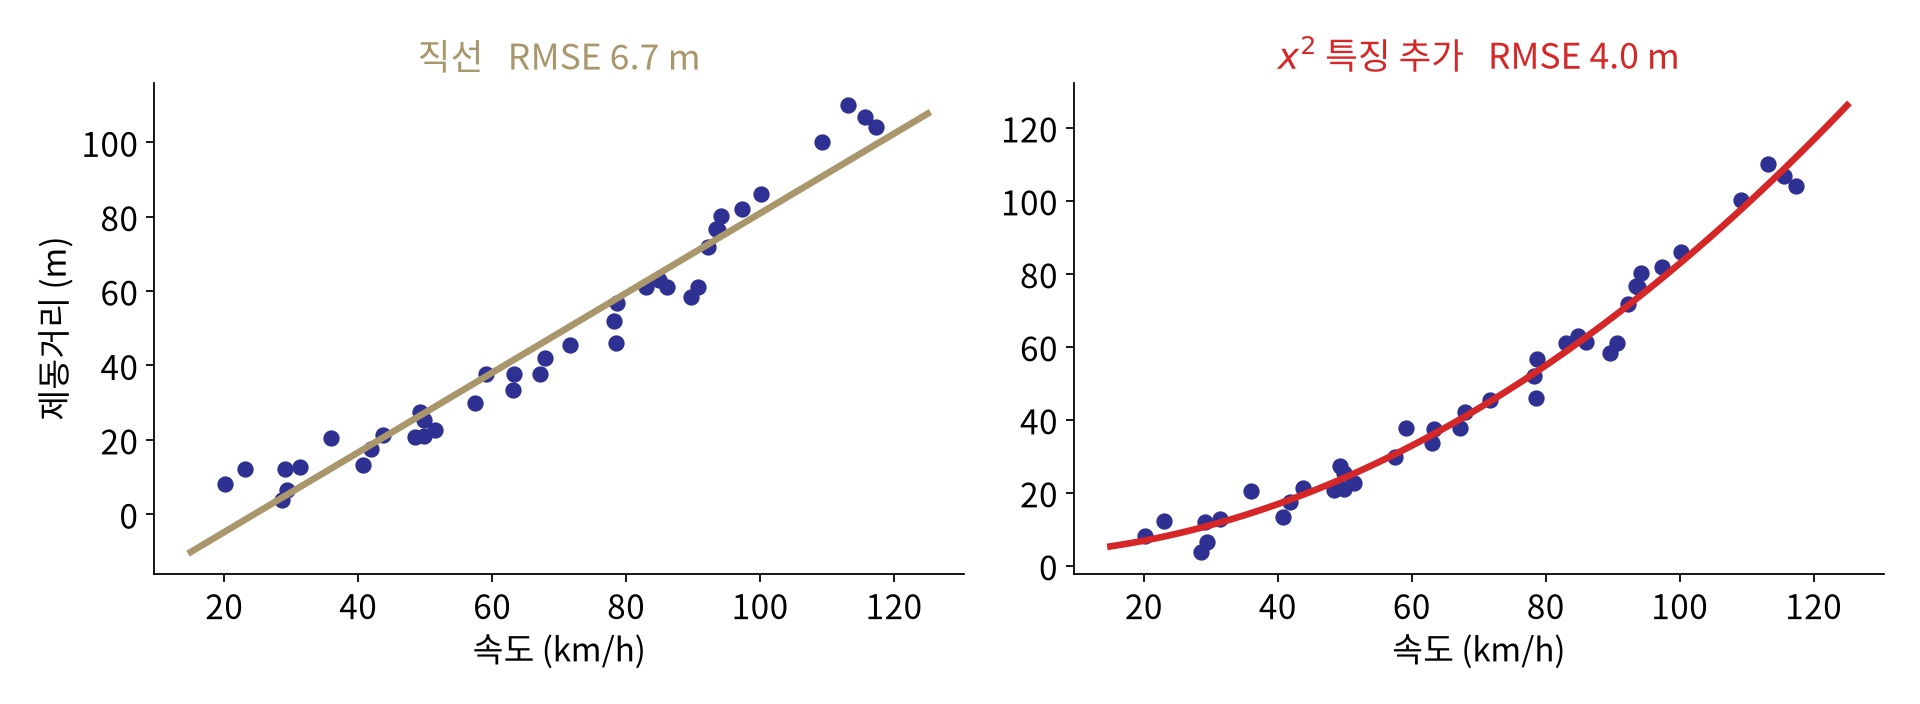
\includegraphics[width=0.9\linewidth]{lr_brake.png}\par\vskip0.3em
{\large 속도 $\to$ 제동거리: $x^2$ 을 \textbf{특징으로 하나 더} 넣으면 \kb{RMSE 6.7 m $\to$ 4.0 m}}
\vfill
\note{이번에는 자동차 속도와 제동거리입니다. 빠를수록 제동거리가 더 가파르게 늘어나는 곡선입니다. 직선으로는 RMSE 6.7미터인데, 속도의 제곱을 특징으로 하나 더 넣어서 h는 w0 더하기 w1 x 더하기 w2 x 제곱으로 바꾸면 4.0미터로 줄어듭니다. 곡선을 그렸는데 이것도 선형회귀입니다. 왜 그럴까요?}
\end{frame}

% --- 선형의 뜻
\begin{frame}{``선형''은 $w$ 에 대해 선형이라는 뜻}
\vfill
\centering
{\Large\[ h(x) = w_0 + w_1\,\underbrace{x}_{\text{feature 1}} + w_2\,\underbrace{x^2}_{\text{feature 2}} \]}\vskip0.6em
{\large $x^2$ 을 새 열로 미리 계산해 두면, $w$ 에 대해서는 여전히 \kb{곱하고 더하기}뿐}\\[0.6em]
{\small 비용 $J$ 도 여전히 그릇 모양 $\to$ 경사하강법 그대로 \pref{gd}}\\[0.8em]
\kq{$h = w_0 + \sin(w_1 x)$ 는? $\to$ $w$ 에 대해 선형이 아니다}
\vfill
\note{선형회귀의 선형은 x에 대해 직선이라는 뜻이 아니라, 가중치 w에 대해 선형이라는 뜻입니다. x 제곱을 미리 계산해서 새 열로 붙여 두면, 모델은 여전히 특징에 w를 곱해서 더하는 것뿐입니다. 그래서 비용 J도 그릇 모양 그대로고, 경사하강법도 그대로 씁니다. 반대로 w가 사인 안에 들어가면 w에 대해 선형이 아니라서 선형회귀가 아닙니다.}
\end{frame}

% --- 로그 변환
\begin{frame}{점점 덜 늘어나면: 로그 변환}
\vfill
\centering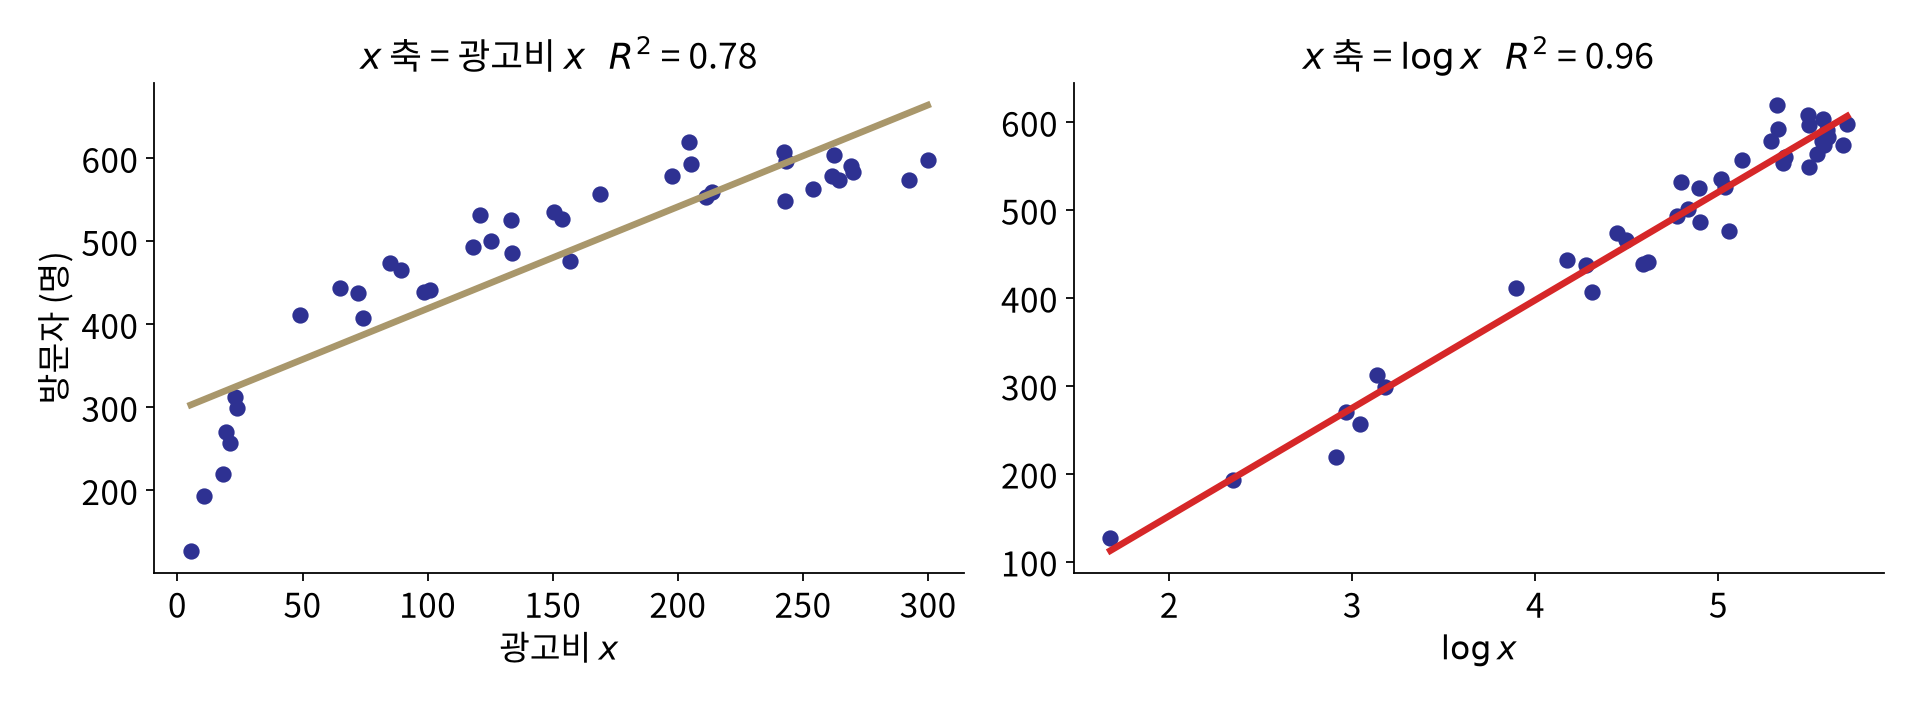
\includegraphics[width=0.9\linewidth]{lr_log.png}\par\vskip0.3em
{\large 광고비 $\to$ 방문자: $x$ 대신 $\log x$ 를 넣으면 \kb{$R^2$ 0.78 $\to$ 0.96}}
\vfill
\note{광고비와 방문자 수입니다. 처음에는 광고비를 늘리면 방문자가 쑥쑥 늘지만, 점점 덜 늘어납니다. 이럴 때는 x 대신 로그 x를 특징으로 넣습니다. 오른쪽처럼 가로축을 로그로 바꾸면 점들이 거의 일직선이 되고, R 제곱이 0.78에서 0.96으로 오릅니다. 이것도 w에 대해서는 선형이니까 선형회귀입니다.}
\end{frame}

% --- 과적합
\begin{frame}{차수를 계속 올리면: 과적합}
\vfill
\centering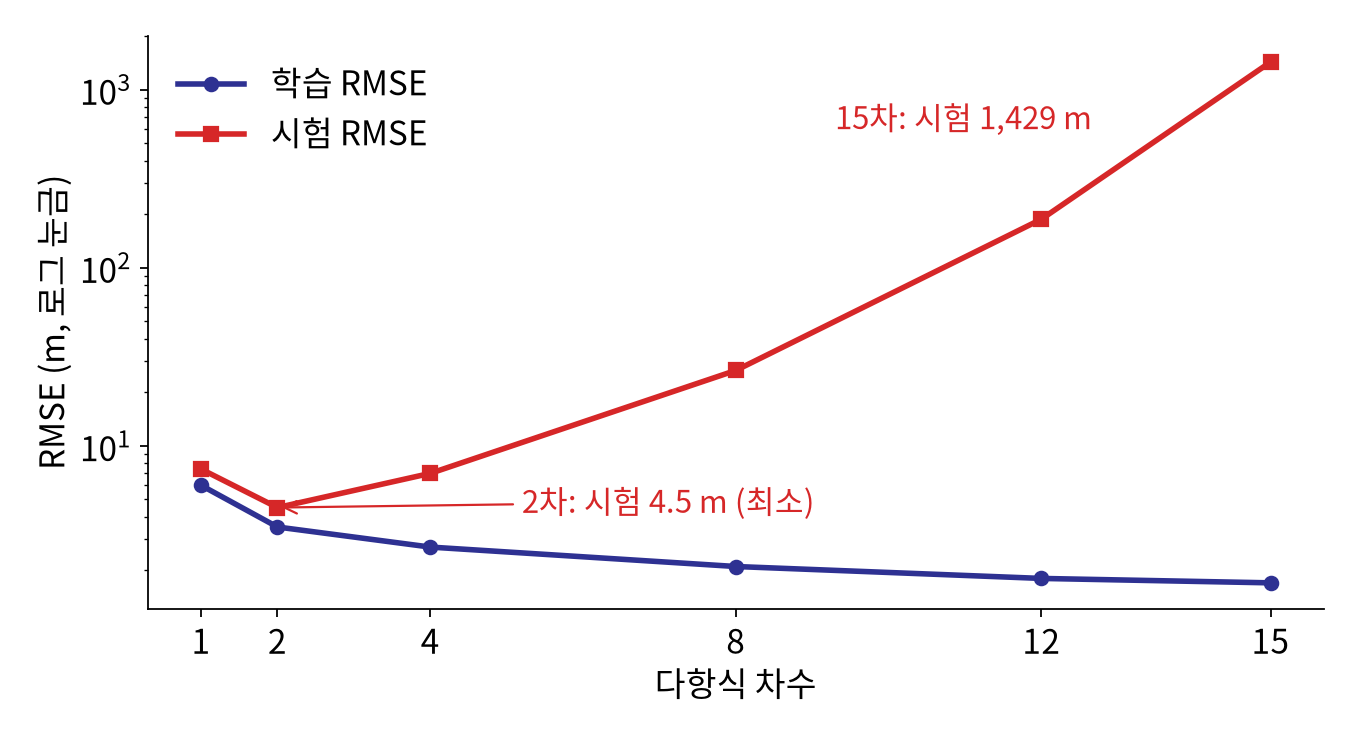
\includegraphics[width=0.62\linewidth]{lr_degree.png}\par\vskip0.3em
{\large 학습 오차는 계속 줄지만, \kq{처음 보는 데이터(시험) 오차는 폭발}한다}
\vfill
\note{그러면 x 세제곱, 네제곱, 계속 넣으면 더 좋아질까요? 제동거리 데이터를 반으로 나눠 반으로 학습하고 나머지 반으로 시험해 봤습니다. 파란 학습 오차는 차수를 올릴수록 계속 줄어듭니다. 그런데 빨간 시험 오차는 2차에서 4.5미터로 가장 작고, 그 뒤로 커져서 15차에서는 1,429미터가 됩니다. 학습 데이터를 외워 버린 겁니다. 이걸 과적합이라고 하고, 5주차 정규화에서 다시 다룹니다.}
\end{frame}

\section{연습}
% --- 문제풀이
\begin{frame}{문제풀이}
\vfill
\begin{enumerate}
\item 데이터 $(1,3), (2,5), (3,7)$, 모델 $h = w_0 + w_1 x$, 지금 $w_0 = 0,\ w_1 = 2$.\\
(a) 세 오차 $h - y$ 는? \; (b) $J$ 는? \; (c) $\partial J/\partial w_0$, $\partial J/\partial w_1$ 는? \; (d) $\eta = 0.1$ 로 한 걸음 가면?\vskip0.8em
\item 다음 중 선형회귀로 풀 수 있는 모델은? \; (a) $w_0 + w_1 x + w_2 x^3$ \; (b) $w_0 + w_1 \log x$ \; (c) $w_0 + e^{w_1 x}$\vskip0.8em
\item 학습 RMSE 는 계속 줄고 시험 RMSE 는 늘어난다. 무슨 일이 일어나고 있나?
\end{enumerate}
\vfill
\note{1번 답. 예측이 2, 4, 6이니 오차는 모두 마이너스 1입니다. J는 2m분의 1 곱하기 오차 제곱의 합, 6분의 1 곱하기 3, 0.5입니다. w0 기울기는 오차의 평균 마이너스 1, w1 기울기는 오차 곱하기 x의 평균, 마이너스 1, 2, 3의 평균이라 마이너스 2입니다. 한 걸음 가면 w0는 0 빼기 0.1 곱하기 마이너스 1로 0.1, w1은 2 빼기 0.1 곱하기 마이너스 2로 2.2입니다. 2번 답. a와 b는 w에 대해 선형이라 선형회귀, c는 w1이 지수 안에 있어서 아닙니다. 3번 답. 학습 데이터를 외우는 과적합입니다.}
\end{frame}

% --- 실습
\begin{frame}{실습}
\vfill
\centering\begin{tabular}{rl}
\large 1 & 경사하강법 직접 구현: 기울기 두 줄 채우기 $\to$ 7시간 75.3점 재현, 학습률 바꿔 발산 보기\\[0.5em]
\large 2 & 실제 자동차 데이터: 마력 $\to$ 연비, 직선 vs $x^2$ vs $\log x$ 의 $R^2$ 비교\\[0.5em]
\large 3 & 같은 데이터로 차수 올리기: 학습 / 시험 오차로 과적합 찾기
\end{tabular}\vskip1em
Auto MPG (자동차 398대, UCI) \\[0.4em]\href{https://colab.research.google.com/github/SuminHan/book-ml/blob/main/slides/ml1/week01/2_linear_regression/lab/linear_regression.ipynb}{\textcolor{ksagolddk}{▶ Colab에서 실습 노트북 열기}}
\vfill
\note{실습은 세 부분입니다. 첫째, 오늘 본 기울기 두 줄을 직접 채워서 경사하강법을 구현하고, 7시간 75.3점을 재현합니다. 학습률을 키워서 발산도 직접 봅니다. 둘째, 실제 자동차 398대의 마력과 연비 데이터에서 직선, 제곱 특징, 로그 변환 중 무엇이 가장 잘 맞는지 비교합니다. 셋째, 같은 데이터로 차수를 올려 가며 과적합이 언제 시작되는지 찾습니다.}
\end{frame}

\section{정리}
% --- 뼈대 다시: 오늘 채운 네 칸
\begin{frame}{오늘 채운 네 칸}
\vfill
\centering
\recipe{{\small (공부 시간, 점수)}\\{\small 30쌍}}{{\small 직선}\\{\small $w_0 + w_1 x$}}{{\small 오차 제곱 평균}\\{\small $J(w_0, w_1)$}}{{\small 경사하강법}\\{\small $w$ 를 고친다}}\par\vskip0.8em
{\large 다음은 \kb{모델과 손실만 바꿔 끼운다}: 로지스틱회귀, 신경망 \ldots \pref{recipe}}
\vfill
\note{처음에 본 학습의 뼈대 네 칸을 오늘 다 채웠습니다. 데이터는 학생 30명의 공부 시간과 점수, 모델은 직선 w0 더하기 w1 곱하기 x, 손실함수는 오차를 제곱해서 평균 낸 J, 최적화는 경사하강법입니다. 다음 주 로지스틱회귀와 뒤에서 배울 신경망도 이 뼈대는 그대로 두고 모델과 손실만 바꿔 끼웁니다.}
\end{frame}

% --- 정리
\begin{frame}{정리}
\vfill
\centering\large\begin{tabular}{l}
풀기 전에 \kb{다섯 칸}: 한 행 · 입력 · 출력 · 평가지표 · 베이스라인\\[0.5em]
모델 \quad $h = w_0 + w_1 x$ \qquad 비용 \quad 오차 제곱의 평균 $J$\\[0.5em]
경사하강법 \quad 기울기 반대로 한 걸음, 학습률은 적당히\\[0.5em]
곡선도 선형회귀 \quad $x^2$, $\log x$ 를 특징으로 ($w$ 에 대해 선형)\\[0.5em]
차수를 너무 올리면 과적합 \quad 시험 오차로 확인
\end{tabular}
\vfill
\note{정리합니다. 선형회귀는 직선 h를 긋고, 오차 제곱의 평균인 비용 J를 재고, 경사하강법으로 J의 바닥을 찾습니다. 학습률은 적당히 골라야 합니다. 곡선 데이터도 x 제곱이나 로그 x를 특징으로 넣으면 선형회귀로 풀 수 있습니다. 선형은 w에 대해 선형이라는 뜻이니까요. 다만 차수를 너무 올리면 과적합이 생기니, 학습에 쓰지 않은 시험 데이터로 확인해야 합니다.}
\end{frame}
\end{document}
